% !TEX root = ../my-thesis.tex
%

\chapter{Banc de test}
\label{sec:Benchmark}

%\cleanchapterquote{Un petit chapitre pour le doctorant, un grand chapitre pour l'humanité}{Doctorant anonyme}{(Citation temporaire)}

\section{Motivations}
\label{sec:Benchmark:Motivations}

\newV{Comme nous l'avons vu dans le chapitre précédent, choisir un filtre de rehaussement pour une application spécifique à partir de la littérature n'est pas simple.} La littérature permet d'avoir une vision globale sur les filtres de rehaussement de vaisseaux sanguins et présente de nombreux exemples d'applications. Cependant, l'incorporation des filtres dans une chaîne de traitements dilue l'évaluation de leur impact réel sur la segmentation. Elle rend aussi plus difficile le choix d'un filtre et de ses paramètres optimaux pour une modalité et un organe spécifiques. De plus, les métriques de références varient aussi entre deux publications ajoutant à la difficulté d'établir une comparaison. Il est donc nécessaire de proposer une base de
 d'évaluation unifiée (Fig. \ref{fig:problematics}).

\begin{figure}[!ht]
  \captionsetup[subfigure]{justification=centering}
  \begin{subfigure}{\textwidth}
    \centering
  \adjincludegraphics[width=0.32\textwidth,trim={{0.12\width} {0.1\height} {0\width} {0.1\height}},clip]{Images/filters_variation_gt.png}
  \caption{Vérité terrain}
  \end{subfigure}
  \begin{subfigure}{\textwidth}
  \adjincludegraphics[width=0.32\textwidth,trim={{0.12\width} {0.1\height} {0\width} {0.1\height}},clip]{Images/antiga_02_08_15.png}
  \adjincludegraphics[width=0.32\textwidth,trim={{0.12\width} {0.1\height} {0\width} {0.1\height}},clip]{Images/antiga_05_05_15.png}
  \adjincludegraphics[width=0.32\textwidth,trim={{0.12\width} {0.1\height} {0\width} {0.1\height}},clip]{Images/antiga_07_03_15.png}
  \caption{Frangi}
  \end{subfigure}
  \\
  \begin{subfigure}{\textwidth}
  \adjincludegraphics[width=0.32\textwidth,trim={{0.12\width} {0.1\height} {0\width} {0.1\height}},clip]{Images/jerman_1.png}
  \adjincludegraphics[width=0.32\textwidth,trim={{0.12\width} {0.1\height} {0\width} {0.1\height}},clip]{Images/jerman_04.png}
  \adjincludegraphics[width=0.32\textwidth,trim={{0.12\width} {0.1\height} {0\width} {0.1\height}},clip]{Images/jerman_01.png}
  \caption{Jerman}
  \end{subfigure}
  \\
  %missing RORPO_50_15_4.png....
  \begin{subfigure}{\textwidth}
  \adjincludegraphics[width=0.32\textwidth,trim={{0.12\width} {0.1\height} {0\width} {0.1\height}},clip]{Images/RORPO_50_15_4.png}
  \adjincludegraphics[width=0.32\textwidth,trim={{0.12\width} {0.1\height} {0\width} {0.1\height}},clip]{Images/RORPO_51_25_3.png}
  \adjincludegraphics[width=0.32\textwidth,trim={{0.12\width} {0.1\height} {0\width} {0.1\height}},clip]{Images/RORPO_100_15_3.png}X
  \caption{RORPO}
  \end{subfigure}
  \caption{Illustration de l'application de différents jeux de paramètres pour plusieurs filtres de rehaussement. Il est difficile de choisir laquelle de ces paramétrisations est la plus apte pour une segmentation sans évaluation quantitative.}
  \label{fig:problematics}
\end{figure}

Dans ce chapitre, nous abordons la conception d'un banc de test permettant l'étude quantitative des filtres de rehaussement. Notre banc de test permet d'appliquer successivement plusieurs \newV{instances de filtres sur une même base de données. Il facilite ainsi l'étude de l'impact des variations des paramètres d'un filtre.} Le résultat des filtrages est ensuite seuillé et les métriques d'évaluations sont calculées dans des zones d'intérêt définies par l'utilisateur. Une fois les métriques collectées, celles-ci peuvent être exploitées indépendamment par des outils de traitement de données. Son fonctionnement est illustré dans la Fig. \ref{fig:schéma banc de test}

La création de notre banc de test passe par la construction d'une interface de filtres unifiée, la construction des jeux de données, la création de zones d'évaluation et le choix des métriques d'évaluation. Cette construction s'est réalisée de manière itérative au fur et à mesure des observations faites durant les expériences d'analyse des filtres et dont les résultats sont présentés dans le chapitre \chapAnalysisN{}.

Avant de décrire chacune de ces étapes, il est nécessaire de mentionner les travaux existants l'évaluation des filtres de rehaussement de vaisseaux.

\tikzstyle{capNode} = [rectangle, rounded corners, minimum width=3cm, minimum height=1cm,text centered, draw=black]
\tikzstyle{capNodeRed} = [rectangle, rounded corners, minimum width=3cm, minimum height=1cm,text centered, draw=red]
\tikzstyle{cNode} = [circle, minimum width=1cm, minimum height=1cm, text centered, draw=black, fill=white!30]
\tikzstyle{arrow} = [thick,->,>=stealth]

\begin{figure}[!ht]
  \centering
  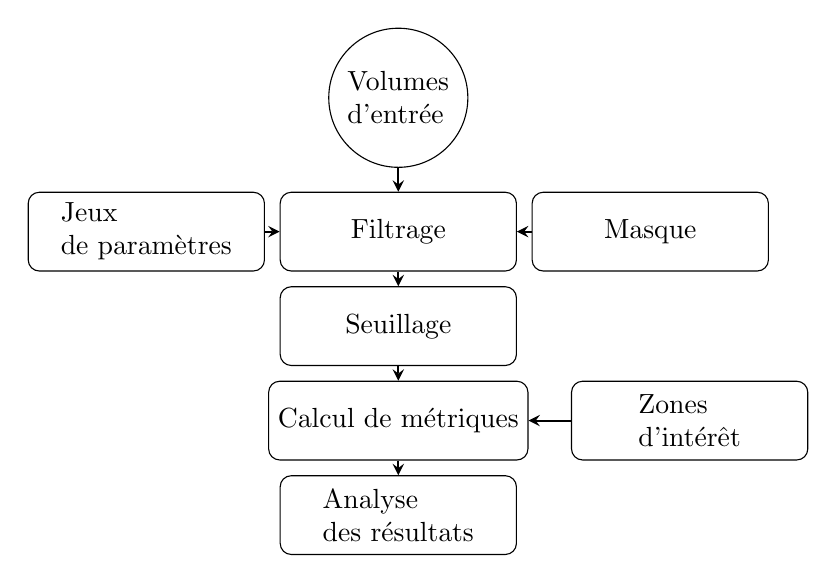
\begin{tikzpicture}[node distance=1.2cm]
    \node (input)[cNode,align=left] {Volumes \\ d'entrée};
    \node (filtrage)[capNode, below of=input,align=left,yshift=-0.5cm] {Filtrage};
    \node (parametres)[capNode, left of=filtrage,align=left,xshift=-2cm] {Jeux \\ de paramètres};
    \node (Masques)[capNode, right of=filtrage,align=left,xshift=2cm] {Masque};
    \node (seuillage)[capNode, below of=filtrage, align=left] {Seuillage};
    \node (metriques)[capNode, below of=seuillage, align=left] {Calcul de métriques};
    \node (ZI)[capNode, right of=metriques, align=left,xshift=2.5cm] {Zones \\ d'intérêt};
    \node (traitement)[capNode, below of=metriques, align=left] {Analyse \\ des résultats};
  
    \draw [arrow] (input) -- (filtrage);
    \draw [arrow] (filtrage) -- (seuillage);
    \draw [arrow] (parametres) -- (filtrage);
    \draw [arrow] (Masques) -- (filtrage);
    \draw [arrow] (ZI) -- (metriques);
    \draw [arrow] (seuillage) -- (metriques);
    \draw [arrow] (metriques) -- (traitement);

  \end{tikzpicture}
  \caption{Schéma global du banc de test. Celui-ci présente une architecture simple afin de faciliter la prise en main par d'autres utilisateurs.}
  \label{fig:schéma banc de test}
\end{figure}

\section{Travaux existants}

 Quelques travaux proposent une comparaison entre filtres de rehaussement. Par exemple Sazak et Alharbi et al. \cite{Alharbi2018_TP_2D_3D} \cite{Sazak2019_bowler_hat_2D}  ont proposé une méthode de rehaussement de vaisseaux à base de morphologie mathématique en 2D et 3D. Ce filtre est comparé à d'autres filtres 2D et 3D à base de hessiennes ou de tenseurs de phase. Ces articles donnent toutefois une part importante à l'évaluation qualitative plutôt que quantitative. De plus, ils ne proposent pas de discussion sur l'impact de la paramétrisation des filtres. En 3D, une analyse quantitative des filtres de rehaussement sur un grand nombre de volumes a été réalisée par Manh Luu et al. en 2015 \cite{Luu2015_liver_vesselness_comparison} et Phellan et al. \cite{Phellan2017_Brain_vesselness_comparison} en 2017. Manh Luu et al. avaient rendu leurs travaux public, mais le site internet n'est aujourd'hui plus accessible.

Manh Luu et al. \cite{Luu2015_liver_vesselness_comparison} ont proposé un banc de test sur 51 images tomodensitométriques du foie sans prétraitement des données. Ils ajoutent cependant dans leur chaine de traitement une segmentation à base de croissance de région et une fermeture morphologique pour supprimer les composantes connexes inférieures à 10 voxels. Dans leurs travaux, l'évaluation de la qualité de la segmentation est basée sur des échantillons de marqueurs positionnés manuellement à l'intérieur et autour des vaisseaux (Fig. \ref{fig:ManhLuu_markers}). Entre 300 et 700 points par volumes sont annotés à l'intérieur des vaisseaux et 4 marqueurs du voisinage des vaisseaux sont ajoutés par points internes. Les filtres testés sont Frangi, Sato, Erdt \cite{Erdt2008_liver_vesselness} et les schémas de diffusion HDCS (\textit{Hybrid Diffusion with Continuous Switch}), VED (\textit{Vessel Enhancement Diffusion}) et RPM (\textit{Regularized Perona-Malik}) \cite{Perona1990_RPM}. Les paramètres des filtres sont optimisés sur une sous-section de la base de données. L'optimisation des paramètres est un fait suffisamment rare dans la littérature pour être souligné. Les métriques utilisées pour l'évaluation des filtres sont le rapport signal sur bruit (SNR), le rappel, la justesse et la spécificité.

\begin{figure}[!ht]
  \centering
  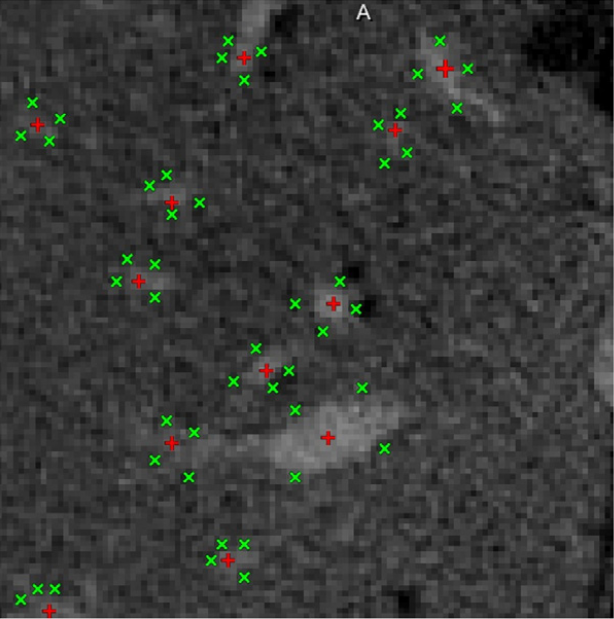
\includegraphics[height=6cm]{Images/ManhLuu_markers.png}
  \caption{Marqueurs utilisés par Manh Luu et al. En rouge, marqueurs de vaisseaux, en vert, marqueurs extérieurs aux vaisseaux. Image issue de \cite{Luu2015_liver_vesselness_comparison}. }
  \label{fig:ManhLuu_markers}
\end{figure}

Phellan et al. \cite{Phellan2017_Brain_vesselness_comparison} proposent quant à eux un banc de test sur 5 images IRM du cerveau et 40 volumes générés avec VascuSynth et l'ajout d'artefacts de tomodensitométrie. Leur chaîne de traitement inclut un prétraitement des données et une segmentation à base de seuillages et d'un filtrage de composantes connexes. Leur méthode d'analyse repose sur des vérités terrains binaires du réseau vasculaire entier et sur l'évaluation du diamètre des vaisseaux. De plus, Phellan et al. considèrent que la détection est plus importante que la précision des contours à l'étape du rehaussement. Ils définissent donc une zone d'acceptation dans laquelle les voxels ne participent pas à la métrique (Fig. \ref{fig:Phellan_acceptance_zone}). Les filtres évalués par Phellan sont Frangi, Sato, Erdt, OOF, RORPO, WTH (\textit{White top hat transform}) \cite{Soille1999_WTH} et les schémas de diffusion HDCS, VED et RPM. Seuls les paramètres d'échelle sont optimisés dans ces travaux, les paramètres intrinsèques par défaut étant fixé par les auteurs. Les performances des filtres sont évaluées grâce au Dice, au MCC, à l'analyse de courbes ROC et à travers une analyse des composantes connexes.

\begin{figure}[!ht]
  \centering
  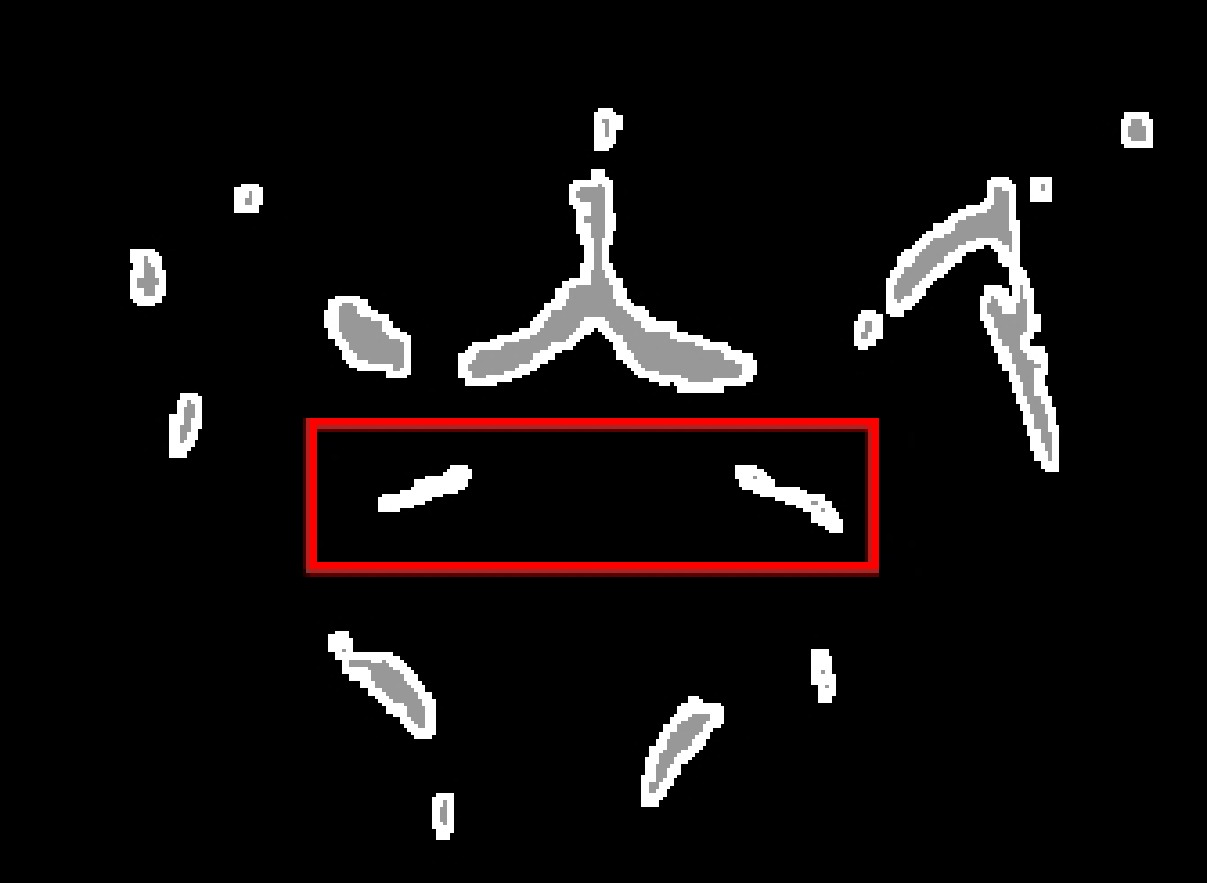
\includegraphics[height=4cm]{Images/Phellan_comparison.jpg}
  \caption{Zone d'acceptation de Phellan définie comme la zone entre l'érosion (gris) et la dilatation (blanc) de la vérité terrain. La bordure réelle des vaisseaux se situe au sein de la zone blanche, mais les métriques ne sont calculées que dans la zone grise. Cette méthode exclut une partie des petits vaisseaux.}
  \label{fig:Phellan_acceptance_zone}
\end{figure}

Ces deux bancs de test proposent des méthodes d'évaluations différentes. Des éléments intéressants pour notre application sont présents dans les deux benchmarks, qui chacun recouvre une partie de nos besoins sans y répondre complètement. Par exemple, l'évaluation de Manh Luu sur le foie n'est pas faite sur une segmentation voxélique. Cette évaluation éparse sur quelques marqueurs dans le voisinage des vaisseaux peut mésestimer des artefacts, comme un rehaussement bruité à la surface des vaisseaux. Le travail de Phellan et al. est réalisé sur le cerveau sans optimisation des paramètres. Des filtres récents ne sont pas évalués, car ils sont postérieurs aux publications. 

Nous souhaitions pouvoir évaluer les filtres sur des zones spécifiquement définies par l'utilisateur telles que les bifurcations des vaisseaux. Ces zones sont en effet connues pour être plus faiblement rehaussées sans que la littérature n'apporte de résultats quantifiables. Une analyse du rehaussement par taille de vaisseaux n'est pas non plus disponible pour le foie. C'est pourquoi nous avons voulu créer notre propre banc de test \newV{et mettre en pratique son utilisation pour des données présentant des contraintes similaires à l'imagerie du foie}. Nous avons voulu éviter de \newV{rencontrer les mêmes limitations} que les travaux précédents en proposant un cadre suffisamment généraliste pour s'accommoder de différentes modalités et suffisamment modulaire afin que la prise en main du banc de test par d'autres utilisateurs soit possible.

La conception de notre banc de test a été guidée par plusieurs axes majeurs.
  
\newV{Le choix du type de vérité terrain pris en charge par notre banc de test a été le premier axe de conception. Comme présenté dans le chapitre \ref{sec:contexte}, nous avions le choix entre segmentation voxélique et segmentation par ligne centrale. Une troisième option telle que l'utilisation de marqueurs, expérimenté par Manh Luu, nous a paru trop éparse pour rendre compte de la totalité du profil du rehaussement. Pour les mêmes raisons, nous avons écarté l'utilisation de vérités terrains à base de ligne centrale. Nous avons donc naturellement choisis de prendre en charge des segmentations et vérités terrains voxéliques dans notre banc de test. Ce choix s'est par la suite avéré le bon, puisque nos jeux de données pré-traités ont été beaucoup partagés au seins du projet ANR.}

\section{Homogénéisation des filtres}
\label{sec:Filtres}

Former une base homogène de filtres n'est pas une tâche simple. Celle-ci nécessite la recherche de code existant ou d'implémenter les filtres en se basant sur la méthodologie de l'article original.

Réaliser l'implémentation d'un filtre à partir des indications de l'auteur est parfois complexe, car il doit souvent se soumettre à un exercice de concision lors de la publication de ses travaux. L'auteur va donc à l'essentiel et certains détails d'implémentation peuvent être omis. La difficulté peut aussi survenir d'un problème de compréhension de la part du lecteur auquel s'ajoute parfois la barrière de la langue. Il faut donc être particulièrement attentif à la compréhension et à la vérification des hypothèses afin d'implémenter correctement les filtres. 

La collecte d'implémentations existantes n'est pas non plus évidente. En effet, il est possible que plusieurs versions d'un algorithme existent. Il est alors nécessaire de vérifier le code en détail. Certaines implémentations peuvent présenter des interfaces différentes de l'article original et nécessiter un travail de traduction d'une interface à l'autre. Il arrive aussi que des codes soient disponibles, mais avec une dette technologique importante suite à l'évolution des logiciels ou des librairies nécessaires à leur fonctionnement. Il est aussi possible que des implémentations ajoutent des améliorations non documentées dans les articles originaux, ce qui peut être problématique dans les travaux de comparaison. Enfin, la multiplicité des langages, des librairies et des logiciels sur lesquels sont déployés les filtres accroît le temps dédié à cette tâche. Ce travail est souvent réalisé de manière isolée par un chercheur, un doctorant, ou un stagiaire pour leurs expériences personnelles et ne profite pas à la communauté travaillant sur le sujet. Il doit alors reprendre de lui-même la totalité de ce travail à chaque introduction d'une nouvelle méthode.

Dans nos travaux, nous avons sélectionné, adapté et implémenté sept filtres qui répondent tous à une problématique spécifique du rehaussement (Tab. \ref{Tab:available_vesselness}). La diversité de leur origine est résumée dans la table \ref{Tab:origins_vesselness}. Il a été choisi d'implémenter ces filtres et d'effectuer les modifications nécessaires pour les filtres existants en C++ avec la librairie ITK. Le C++ est particulièrement connu pour sa rapidité, un élément crucial pour des applications 3D qui doivent traiter un nombre important de voxels. La librairie open source ITK (Insight ToolKit), développée par Kitware Inc. depuis 2001, est la plus importante librairie de traitement d'images médicales. Elle fournit un ensemble de briques algorithmiques déjà implémentées et présente l'avantage de lire nativement une grande diversité de formats d'images médicales, ce qui est un atout pour la diffusion de notre banc de test.

Cette librairie s'appuie sur une communauté active et connait des mises à jour régulières. C'est à la fois un avantage, pour la correction de bugs et l'introduction de nouveaux algorithmes mais aussi un inconvénient, car la dette technologique s'accumule plus rapidement à cause de cycles plus courts entre deux versions.


\begin{table}
    \begin{center}
      \resizebox{\textwidth}{!}{
  \begin{tabular}{l|l|l}
  Méthode   &  Idée principale                                                                       & Date \\ \hline  \hline 
  Sato      & Reconnexion des vaisseaux, contrôle du bruit                                         & 1997 \\ \hline
  Frangi    & Contrôle sur l'atténuation des structures en plateau et en blob                     & 1998 \\ \hline
  Meijering & Détection de fines structures allongées                                             & 2004 \\ \hline
  OOF       & Limitation du débordement des réponses lié à l'espace d'échelles gaussien             & 2010 \\ \hline
  Jerman    & Contrôle de l'homogénéité des réponses des vaisseaux                                 & 2016 \\ \hline
  Zhang     & Pré-traitement pour limiter le rehaussement des bordures du foie (TDM foie)          & 2018 \\ \hline
  RORPO     & Détection par chemins et différentiation des vaisseaux par vote sur les orientations & 2018  
  \end{tabular}
  }
  \end{center}
  \caption{Méthodes disponibles et idées principales guidant leur conception.}
  \label{Tab:available_vesselness}

  \end{table}

  \begin{table}
    \begin{center}
      \resizebox{\textwidth}{!}{
        \begin{tabular}{l|l|l|l}
            Méthode   &  Provenance                                     & État \\ \hline  \hline 
            Sato      & Librairie ITK (C++)                             & prêt à l'emploi \\ \hline
            Frangi    & Librairie ITK (C++)                             & prêt à l'emploi \\ \hline
            Meijering & Github (Matlab), scipy                          & pondération proposée ne respectant pas l'article original.  \\ \hline
            OOF       & Site de l'auteur (Matlab), insight journal (C++)& obsolète \\ \hline
            Jerman    & Github de l'auteur (Matlab)                     & prêt à l'emploi \\ \hline
            Zhang     & Non disponible                                  & non implémenté \\ \hline
            RORPO     & Github de l'auteur (C++)                        & prêt à l'emploi  
        \end{tabular}
      }
    \end{center}
    \caption{Origine des méthodes. La diversité des provenances et l'ancienneté du code complique la mise en oeuvre d'une comparaison des filtres.}
    \label{Tab:origins_vesselness}
  \end{table}

\newV{Une fois ces filtres collectés, il a été nécessaire de les standardiser afin de pouvoir former une base commune de comparaison. Cette standardisation englobe la redéfinition du domaine de sortie des filtres ainsi que la manière d'incorporer des masques de filtrage.}

\subsection{Redéfinition du domaine de sortie des filtres}

\newV{Le rehaussement de vaisseaux est parfois présenté comme une carte de chaleur ou de probabilité pour laquelle une mesure de la tubularité locale est associée à chaque voxel. La mesure de tubularité n'est toutefois pas définie sur le même interval pour chaque filtre.}

Pour le filtre de Frangi, la mesure de tubularité est définie entre 0 et 1 par conception. Cette propriété n'est pas nécessairement partagée par d'autres filtres. Parmis notre sélection, seuls Jerman, Zhang et Meijering fournissent une réponse définie sur cet intervalle. La réponse de Sato est définie sur $[0,+\infty]$, tout comme celle d'OOF. RORPO est un cas particulier, car l'intensité de sortie du filtre dépend de l'intensité maximum de l'image initiale. En effet, RORPO se base sur des ouvertures morphologiques dont la définition est bornée par le domaine de l'image. 

\newV{La sortie des filtres est nécessairement dépendante des données d'entrées. Les filtres dont les sorties sont définies sur $[0,+\infty]$ sont donc en pratique bornés par la variation maximale d'intensité des images. Une solution envisageable serait donc de normaliser les images d'entrée. Il nous a cependant semblé plus pratique de normaliser la sortie des filtres.}

Nous avons choisi pour Sato et OOF de normaliser la réponse de sortie en fonction de la plus grande valeur de sortie du filtre :

\begin{equation}
  \frac{I_{rehaussement}(x)} {\max(I{rehaussement}(x))}
\end{equation}

Pour RORPO dont la sortie est liée à l'intensité de l'image d'entrée, la normalisation prend la forme $ \frac{I_{rehaussement}(x)} {\max(I(x))} $.

\newV{La nature de RORPO en fait un filtre difficile à intégrer à notre banc de test. Avec RORPO, un voxel est considéré comme tubulaire si un ensemble de chemins d'orientations similaires passent par ce voxel. RORPO ne définit donc pas de degré de tubularité à proprement parlé et produit soit des voxels non tubulaires à valeur nulle, soit des voxels tubulaires à intensité proche de leur intensité initiale (les opérateurs $\min$ et $\max$ de l'ouverture ne conservent pas toujours l'intensité initiale du voxel). Cette "segmentation en niveaux de gris" force l'utilisation d'une normalisation basée sur les intensités des voxels tubulaires pour passer à une carte de probabilité nécessaire pour l'utilisation de notre banc de test. Cette procédure a un impact non négligeable sur le résultat des expériences présentées dans le chapitre suivant.}

Une attention particulière doit être portée aux types d'images pris en charge par l'implémentation des filtres. Les images 2D classiques sont souvent composée de canaux de 8 bits qui expriment 256 niveaux $[0,255]$ par canal. Habituellement, une image en niveau de gris est composée d'un seul canal, une image couleur de 3 canaux (rouge, vert, bleu) et plus pour une image multispectrale. 

La dynamique des images médicales abdominales n'est pas commune. Elles possèdent la plupart du temps un seul canal avec parfois une dynamique de niveaux de gris plus élevée de 16 ou 32 bits. Des valeurs négatives peuvent aussi être présentes, comme pour la tomodensitométrie présentée au chapitre \chapContextN. Il faut donc s'assurer que les filtres prennent bien en compte les mêmes types d’images. Un même filtre peut en effet produire des résultats différents selon la précision des images (8 bits vs. 32 bits). Par exemple, l'implémentation de RORPO ne supporte que des valeurs de pixels positifs et nécessite de faire une translation des niveaux de gris négatifs sous peine d'obtenir des comportements non définis.

\subsection{Utilisation de masques}

Il peut souvent être utile de ne traiter qu'une partie de l'image, par exemple lorsque l'utilisateur ne veut rehausser les vaisseaux que d'un organe en particulier. La manière la plus simple est de définir un masque binaire de taille équivalente à l'image. On renseigne pour chaque voxel s'il appartient à la zone à traiter (1 ou 255) ou s'il n'y appartient pas (0). 

\newV{Différentes stratégies d'application du masque sont possibles. En fonction du filtre, celles-ci peuvent avoir un impact sur le temps de calcul ou la qualité du rehaussement. On peut en effet distinguer deux catégories de filtres de rehaussement qui demandent des stratégies différentes de masquage : Les filtres à information locale (ou semi-locale) et les filtres à information locale et globale.}

\newV{Les filtres à information locale ne considèrent le rehaussement que par rapport à des mesures effectuées dans un voisinage local. Ce voisinage est défini par la taille de la gaussienne pour les méthodes à espace d'échelles gaussien et par la taille de l'élément structurant pour les méthodes à base de morphologie. Les filtres à information locale sont Frangi, Sato et OOF. RORPO est un filtre semi-local, car l'élément structurant non isotrope peut-être long \cite{Merveille2018_curvilinear}.}

Les filtres à information globale sont Meijering, Jerman et Zhang. Meijering et Jerman/Zhang nécessitent la plus petite valeur propre (équivalent à la plus grande valeur propre négative en valeur absolue) de la zone sur laquelle est appliqué le rehaussement. Le pré-filtrage de Zhang nécessite lui aussi une information globale puisque cette étape repose sur la classification de l'ensemble des pixels de la zone de rehaussement.

\newV{Une première stratégie de masquage consiste à appliquer le masque après le rehaussement. Le filtre est appliqué à toute l'image puis le résultat est masqué  pour ne conserver que le rehaussement de l'organe observé. Cette implémentation a le désavantage de calculer le rehaussement dans des zones non utilisées par la suite, telles que les zones autour du corps du patient. Pour les filtres à information globale, cette manière de masquer à un impact critique sur le résultat du rehaussement. Par exemple pour le filtre de Jerman appliqué au foie, la mesure de rehaussement sera pondérée par les valeurs propres minimales de l'image, donc celle des os (structures intenses), et non celles des vaisseaux.}

\newV{Afin d'éviter ce problème, on peut masquer les filtres avant le rehaussement de vaisseaux. On masque ainsi l'image originale puis on applique le filtre de rehaussement sur l'image masquée. On règle ainsi le problème des filtres à information globale en masquant les structures parasites. On gagne aussi en temps de calcul dans les zones constantes à valeurs nulles qui ne font pas partie de l'évaluation. Ce gain de temps n'est pas négligeable, puisqu'un banc de test applique de multiples fois les filtres sur un grand nombre de volumes 3D. Toutefois, masquer avant le rehaussement créé artificiellement de faux bords en induisant un différentiel d'intensités marqué (voir Fig. \ref{fig:mask_intensity_profile}).}
 
\begin{figure}[!ht]
  \centering
  \adjincludegraphics[width=0.4\textwidth,trim={{0.2\width} {0.1\height} {0.2\width} {0.1\height}},clip]{Images/output_maskedFirst.png}
  \adjincludegraphics[width=0.4\textwidth,trim={{0.2\width} {0.1\height} {0.2\width} {0.1\height}},clip]{Images/output_unmasked.png}
  \adjincludegraphics[width=0.4\textwidth,trim={{0.2\width} {0.1\height} {0.2\width} {0.1\height}},clip]{Images/output_masking_diff.png}
  \caption{Application du masque avant le rehaussement (gauche) et après (droite). La différence (fond gris) des deux masques est visible au centre. Le masque en amont crée un contour artificiellement net que le filtre rehausse.}
  \label{fig:mask_intensity_profile}
\end{figure}

Une stratégie de masque a donc été choisie spécifiquement pour chaque filtre \ref{fig:masks_posible_location}. Ainsi pour Frangi, Sato, OOF, RORPO, le masque est appliqué après rehaussement afin de limiter l'introduction de faux gradients liés au masque.

\begin{figure}[!ht]

  \centering
  %\resizebox{\linewidth}{
    
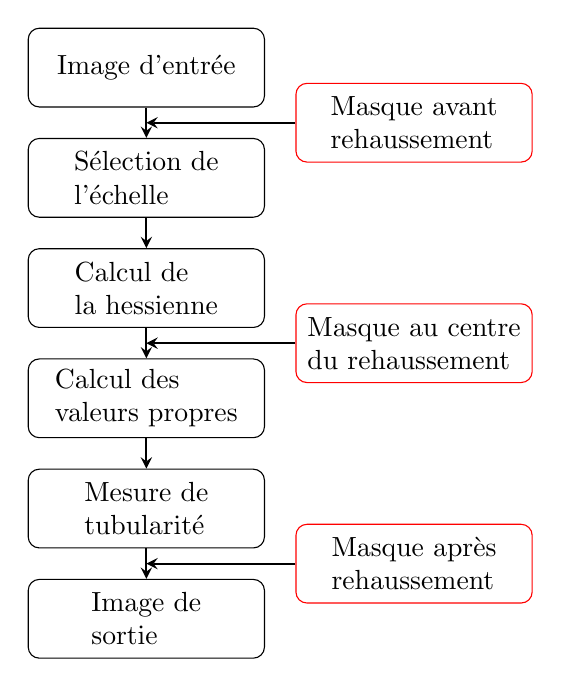
\begin{tikzpicture}[node distance=1.4cm]
  \node (input)[capNode] {Image d'entrée};
  \node (scale_selection)[capNode, below of=input,align=left] {Sélection de \\ l'échelle};
  \node (hessian)[capNode, below of=scale_selection,align=left] {Calcul de \\ la hessienne};
  \node (EV)[capNode, below of=hessian,align=left] {Calcul des \\ valeurs propres};
  \node (vesselness)[capNode, below of=EV,align=left] {Mesure de \\ tubularité};
  \node (output)[capNode, below of=vesselness,align=left] {Image de \\ sortie};

  \draw [arrow] (input) -- (scale_selection) coordinate[midway] (a_input){};
  \draw [arrow] (scale_selection) -- (hessian) coordinate[midway] (a_sc){};
  \draw [arrow] (hessian) -- (EV) coordinate[midway] (a_hessian){};
  \draw [arrow] (EV) -- (vesselness) coordinate[midway] (a_EV){}; 
  \draw [arrow] (vesselness) -- (output) coordinate[midway] (a_Vesselness){};

  \node (p1)[capNodeRed,right of=a_input,xshift=2cm,align=left]{Masque avant \\ rehaussement};
  \node (p2)[capNodeRed,right of=a_hessian,xshift=2cm,align=left]{Masque au centre \\ du rehaussement};
  \node (p3)[capNodeRed,right of=a_Vesselness,xshift=2cm,align=left]{Masque après \\ rehaussement};

  \draw [arrow] (p1) -- (a_input);
  \draw [arrow] (p2) -- (a_hessian);
  \draw [arrow] (p3) -- (a_Vesselness);

  %\draw [arrow] (bestScaleParameter) -| node[anchor=east]{}([shift={(1.3cm,0mm)}]bestScaleParameter.east)|-([shift={(0mm,-1mm)}]computeParams2.west);
\end{tikzpicture}
%}
\caption{Emplacements possibles pour masquer la réponse. Le masque au centre bénéficie des avantages de rapidité de calcul offert par le masque appliqué avant le rehaussement tout en limitant les effets de bords comme le masque après rehaussement.}
\label{fig:masks_posible_location}
\end{figure}

Pour les autres filtres, une stratégie plus complexe a été utilisée. Comme nous avons implémenté nous-même les filtres de Jerman, Meijering et Zhang, nous avons un contrôle plus fin sur l'étape d'application du masque. Afin de combiner les deux propriétés de limitation du temps de calcul et de non-introduction de bordures nettes artificielles, l'opération de masque est introduite entre le calcul de la matrice hessienne et le calcul de ses valeurs propres. Ne sont calculées les valeurs propres que des pixels appartenant au masque tout en calculant la matrice hessienne sur la globalité du volume. On obtient ainsi un compromis tirant parti des avantages entre masque avant et après rehaussement (voir Fig. \ref{fig:smart_mask_effect}).

\begin{figure}[!ht]
  \centering
  \adjincludegraphics[height=6cm,trim={{0.15\width} {0.1\height} {0.2\width} {0.1\height}},clip]{Images/globInfo_noM_loc.png}
  \adjincludegraphics[height=6cm,trim={{0.10\width} {0.05\height} {0.15\width} {0\height}},clip]{Images/globInfo_M_loc.png}
  \adjincludegraphics[height=6cm,trim={{0.15\width} {0.1\height} {0.15\width} {0.1\height}},clip]{Images/globInfo_noM_glob.png}
  \caption{Première ligne : à gauche, filtre de Jerman avec un masque appliqué après le rehaussement. À droite, filtre de Jerman avec un masque appliqué avant le rehaussement. Seconde ligne : rehaussement avant l'application du masque en aval. La limite haute du rehaussement est définie par les structures intenses hors du foie plutôt que par les vaisseaux hépatiques. Dans les deux cas, les mêmes paramètres ont été appliqués.}
  \label{fig:smart_mask_effect}
\end{figure}

Zhang est le filtre le plus complexe. Il nécessite une étape de prétraitement par une K-moyenne pour paramétrer une fonction sigmoïde. Celle-ci sert ensuite à pré-filtrer l'image avant le rehaussement. Dans la méthode originale, le nombre de classes de la K-moyenne est défini par rapport à des images masquées. Cette K-moyenne est donc appliquée sur l'image globale masquée (fond mis à 0) avant le filtrage par sigmoïde. Ensuite la même stratégie de masquage que pour Jerman et Meijering est utilisée. La K-moyenne classique est une opération coûteuse, en particulier lorsqu'elle est effectuée sur un volume 3D. Afin d'éviter un surcoût, nous avons utilisé une K-moyenne à partir d'un quadtree, ce qui réduit significativement le temps de calcul de cette étape.

Les 7 filtres sont implémentés en C++ et reposent sur la librairie ITK. Ceux-ci sont organisés sous forme de CLI ( \textit{command line interface}) indépendants du cadre du banc de test et peuvent être utilisés en dehors de celui-ci. Cela signifie également que n'importe quel nouveau filtre respectant l'interface définie dans le benchmark (c'est-à-dire une entrée, une sortie et un masque optionnel) peut être ajouté de manière transparente à celui-ci.

\section{Pré-traitements des jeux de données}
\label{sec:Benchmark:traitement_des_données}

Dans le bilan du chapitre \chapContextN{} (Sec. \ref{sec:contexte:bilan}), nous avons présenté les bases de données publiques que nous avons sélectionné pour l'analyse des filtres de rehaussement.

Ces trois bases de données sont réparties en deux bases de données réelles, l'Ircad et Bullitt, et une base de données synthétique issue du logiciel VascuSynth \cite{Hamarneh2010_vascuSynth}.

\newV{Ces données ont toutes nécessité des prétraitements afin d'être exploitables dans notre banc de test. Nous décrivons dans les sections qui suivent les itérations principales du traitement effectué sur les données réelles puis sur les données synthétiques.}

\subsection{Traitement des données réelles}

\newV{Les voxels des images IRM et TDM sont des parallélépipèdes. L'acquisition d'une image est effectuée par coupes successives et l'opérateur doit trouver un compromis entre temps d'acquisition et qualité de l'image. Un voxel couvre donc la plupart du temps une zone plus grande dans l'axe Z que dans le plan X-Y. Les algorithmes dépendants de la géométrie sont généralement conçus pour être utilisés sur des images à voxels cubiques, de manière à ce qu'une mesure dans n'importe quelle direction de l'image reste consistante. La plupart des opérations géométriques sont biaisées si elles sont utilisées directement sur des données TDM et IRM. On pourrait envisager de prendre en compte la différence de distance en fonction des axes de l'image, mais cela nécessiterait de ré-implémenter la quasi-totalité des outils algorithmiques que nous utilisons. Il est donc plus simple d'adapter les données directement grâce à un procédé de ré-échantillonnage}.

\newV{La taille des axes d'une image en TDM ou en IRM a une correspondance directe avec une grandeur physique. par exemple, la première image de la base de l'Ircad recouvre un volume de $212.04 \times 172.14 \times 180.8$ mm. Dans ce volume est défini un certain nombre de voxels, ici $372 \times 302 \times 113$. On appelle le rapport du nombre de pixels sur la taille des axes du volume la résolution. Dans un volume de taille fixe, plus le nombre de voxels est élevé et plus la résolution est élevé. Cela implique qu'une mesure plus fine des éléments de l'image est effectuée. À l'inverse, plus le nombre de voxels est faible et plus la résolution est faible. Une mesure plus grossière des structures de l'image est effectuée. Évidemment, cette constatation est relative par rapport à la taille des éléments observés. Par exemple, une résolution au millimètre prêt peut-être adaptée pour observer un organe et ne pas suffire pour l'étude de capillaires.}

L'ensemble des voxels peuvent aussi être considéré comme une grille d'échantillonnage. Une grille de haute résolution possèdera un maillage fin tandis qu'une grille de basse résolution possèdera un maillage large. Dans notre cas, nous voulons changer la résolution de nos images, pour que les voxels soient isotropes pour qu'un pas d'une unité dans une direction aléatoire ai une mesure constante (Fig. \ref{fig:resolution_voxels_shapes}). Dit autrement, nous voulons que l'espacement de la grille d'échantillonnage soit le même, peu importe l'axe considéré.

\begin{figure}[!ht]
  \centering
  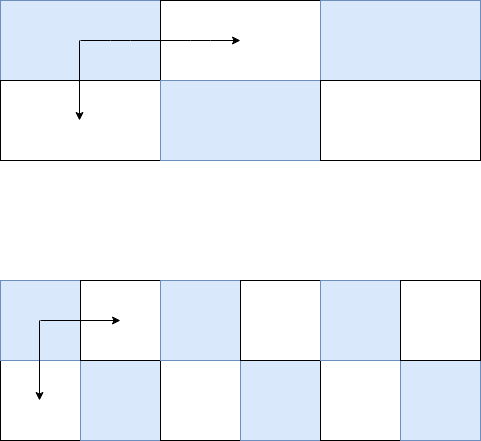
\includegraphics[height=4cm]{Images/resolution_voxels_shape.png}
  \caption{Contrairement à une grille cubique (bas), un pas discret dans une grille formée de parallélépipèdes (haut) n'équivaut pas à un pas discret dans une autre direction. Cette différence peut avoir un impact sur de nombreux algorithmes basés sur la distance (gradients, cartes de distances, etc.).}
  \label{fig:resolution_voxels_shapes}
\end{figure}

Le ré-échantillonnage consiste à re-définir une autre grille d'échantillonnage que celle d'origine. Pour cela, on part de la grille d'échantillonnage originale afin de d'approximer le signal continu sous-jacent. Ensuite, on applique un nouvel échantillonnage sur le signal approximé avec l'espacement désiré. En pratique, on ne reconstruit pas l'ensemble du signal continu, mais pour chaque nouvel échantillon, on détermine sa valeur par interpolation des valeurs existantes voisines. Plusieurs types d'interpolations existent (Fig. \ref{fig:interpolation}) : l'interpolation linéaire (bi-linéaire pour la 2D et tri-linéaire pour la 3D, etc.), l'interpolation par polynômes comme l'interpolation bi-cubique qui utilise un polynôme de degré 2 et l'interpolation à partir de B-Splines. Les interpolations utilisant des polynômes permettent des reconstructions plus fidèles par rapport à des interpolations linéaires, moyennant un coût supplémentaire en calcul. Ce type d'interpolation peut toutefois présenter des instabilités telles que des effets d'oscillation ou l'augmentation artificielle du contraste local (i.e. piqué). L'utilisation de B-Spline permet de limiter ces effets grâce à une formulation polynomiale par partie et continue \ref{Unser1993_bspline}. Dans le reste de nos travaux, les images en niveaux de gris ont été ré-échantillonnées à l'aide d'une interpolation à base de B-spline d'ordre 2. Les images binaires ont été ré-échantillonnées à l'aide d'une interpolation à base de plus proches voisins afin de conserver le caractère binaire des images.


\begin{figure}[!ht]
  \centering
  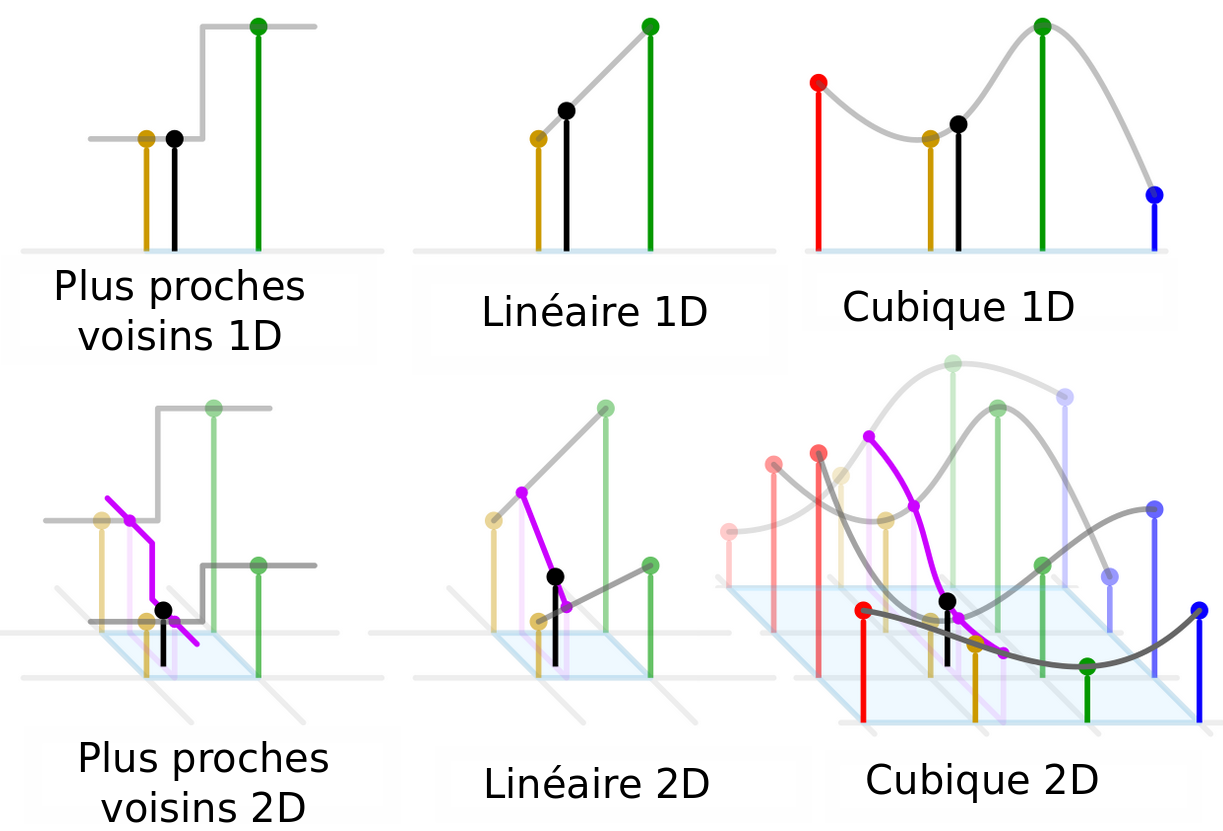
\includegraphics[height=6cm]{Images/Interpolation.png}
  \caption{Différents types d'interpolations. Chaque point peut-être associé à un pixel 1D ou 2D dont l'élévation correspond à l'intensité. Les points de couleur représentent les pixels nécessaires à l'interpolation et le point noir le point interpolé. Les interpolations cubiques (polynôme d'ordre 2) ou B-Spline produisent une reconstruction plus douce qui prend mieux en compte le contexte de variations autour du pixel interpolé.\protect \footnotemark}
  \label{fig:interpolation}
\end{figure}

\footnotetext{Source : \url{https://en.wikipedia.org/wiki/Interpolation}}

Nous avons testé plusieurs résolutions pour rendre les images isotropes. En premier lieu, nous avons ré-échantillonné les images à une résolution normalisée de 1 mm pour chaque axe. Cet échantillonnage a l'avantage, d'avoir une correspondance directe 1 voxel égal à 1 mm, ce qui facilite le paramétrage de l'espace d'échelles des filtres. Un second avantage à cette convention est que le nombre de voxels est largement réduit par rapport au nombre initial de voxels.
Par exemple, pour l'Ircad, l'utilisation de cette convention  réduit la résolution dans les axes X et Y et augmente la résolution de l'axe Z réduisant ainsi significativement le nombre de voxels par volume. Le désavantage de cette méthode est qu'une partie de la géométrie est déformée à par le sous-échantillonnage axial. Il y a ainsi un risque de faire disparaitre de petits vaisseaux ou d'altérer des caractéristiques des vaisseaux comme leur courbure.  Bien que non optimale, nous avons utilisé cette politique lors de nos premières expériences. Les filtres et le banc de test demandent de multiples copies de l'image d'entrée (cadre multi-échelles, masques, vérité terrain, etc.) et la demande en mémoire RAM était un goulot d'étranglement de notre application. Ce choix de résolution permettait d'exécuter notre banc de test sur une machine avec moins de 10 Go de RAM.

Dans un second temps, nous avons opté pour un ré-échantillonnage à la résolution la plus haute de chaque volume qui correspond le plus souvent à la résolution axiale. Par exemple un volume de résolution [0.65 mm, 0.65 mm, 1.5 mm] est ré-échantillonné à une résolution de [0.65 mm, 0.65 mm, 0.65 mm]. De cette manière, aucun axe n'est sous-échantillonné et l'ensemble des détails est préservé et encodé dans des voxels isotropes. L'axe de résolution inférieur est tout de même sur-échantillonné ce qui nécessite une interpolation. On obtient par cette opération des images significativement plus lourdes que les images originales. On impacte donc négativement à la fois la mémoire nécessaire et le temps de calcul des filtres. Cette contrainte s'est toutefois allégée lorsque nous avons eu accès à un cluster de calcul.

Une comparaison des images des deux stratégies est présentée figure \ref{fig:resolution_comparison}.

\begin{figure}[!ht]
  \centering
  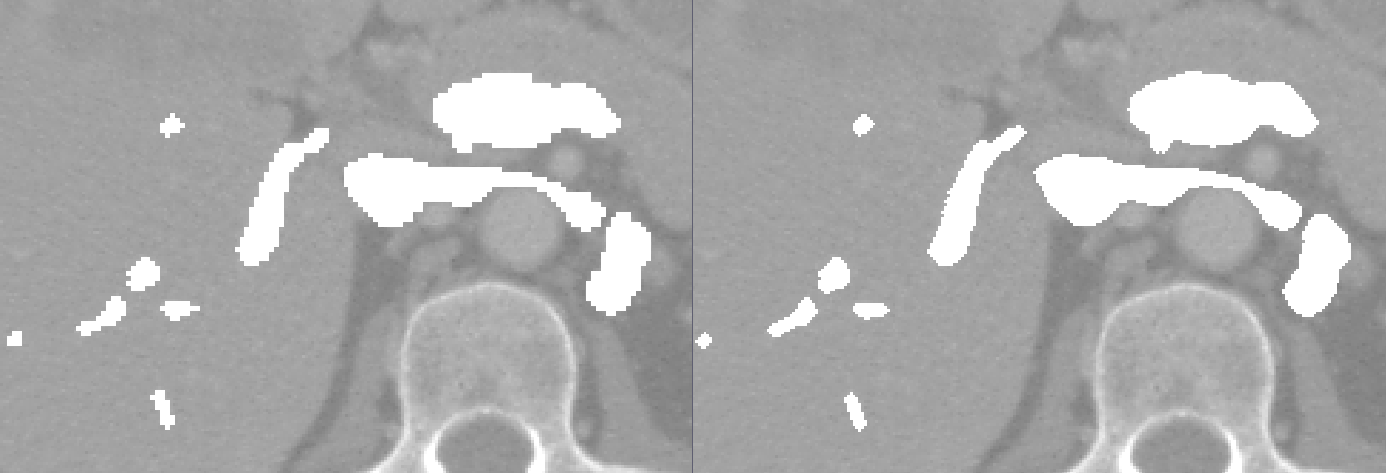
\includegraphics[width=\textwidth]{Images/resolution_111_xxx.png}
  \caption{Illustration des deux stratégies d'échantillonnage : à gauche résolution $1\times1\times1$ mm, à droite résolution $0.57\times0.57\times0.57$ mm. L'image de résolution plus élevée (droite) contient quatre fois plus de voxels ($\sim 27$ Millions) que l'image basse résolution ($\sim 6.6$ Millions) mais la géométrie des vaisseaux est mieux préservée.}
  \label{fig:resolution_comparison}
\end{figure}

Afin de limiter l'augmentation des tailles d'image, nous les avons recadrées pour supprimer le maximum de voxels inutiles, c'est-à-dire ceux en dehors du masque de l'organe. Pour ce faire, nous avons redimensionné les images à la taille de la boîte englobante du masque de l'organe en incluant une bordure de sécurité de $15$ voxels. \newV{Pour les images de foie de l'Ircad, les masques sont souvent formés du masque du foie et de petites composantes connexes parasites. Il est donc nécessaire de faire une analyse de la taille des composantes connexes afin de récupérer la boîte englobante exacte du foie.}

Ce procédé nous a permis de réduire de $43$ \percent{}le nombre de voxels sur l'Ircad et limite l'augmentation moyenne des voxels de Bullitt à $18.7$ \percent. Le gain considérable enregistré sur l'Ircad est dû au fait que le foie représente seulement une petite portion des images abdominales.

Pour la base de données Bullitt, les images d'IRM sont des images destinées à la recherche et sont d'une qualité particulièrement élevée. Une fois un masque du cerveau obtenu, il est très facile de récupérer une grande partie des vaisseaux grâce à un simple seuillage. \newV{Nous avons donc complexifié ces données en renforçant les artefacts IRM de variations d'intensité et le bruit ricien (Fig. \ref{fig:modifications_bullitt}). Les détails de cette modification sont explicités dans la sous-section suivante.}

\begin{figure}[!ht]
  \centering
  \adjincludegraphics[height=7cm,trim={{0.05\width} {0.05\height} {0.05\width} {0.05\height}},clip]{Images/threshold_bullitt.png} \\
  \adjincludegraphics[height=7cm,trim={{0.05\width} {0.05\height} {0.05\width} {0.05\height}},clip]{Images/threshold_bullitt_difficult.png}
  \caption{Segmentation d'un volume de Bullitt par seuillage simple. À gauche, données originales seuillées où la plupart des vaisseaux sont segmentés. À droite, données modifiées. Les vaisseaux sont alors impossibles à récupérer sans inclure une part significative de tissus non vasculaires.}
  \label{fig:modifications_bullitt}
\end{figure}

\subsection{Génération de données synthétiques}

Pour compléter les images réelles, nous avons utilisé le jeu de données synthétiques VascuSynth (Fig. \ref{fig:snap_vascu}) présenté dans le chapitre \chapContext{}. Ce jeu est bi-modale dans le sens où seuls des vaisseaux et un fond nul sont présents. Il présente cependant l'avantage d'être un environnement complètement contrôlé par l'utilisateur et permet d'obtenir des vérités terrains au pixel près. 

\newV{Durant cette thèse, nous avons dans un premier temps travaillé avec le jeu TDM de l'Ircad. Nous avons ensuite utilisé le jeu de données de VascuSynth. Ce n'est que bien plus tard que nous avons ajouté le jeu d'IRM réelles Bullitt à nos expériences. Au moment où nous avons sélectionné VascuSynth, nous avons choisi de simuler des volumes d'IRM du foie.
Les travaux portants sur l'IRM du foie sont bien moins représentés dans la littérature comparé à l'imagerie TDM. L'impact du rehaussement de vaisseaux pour cette modalité est de ce fait très peu étudiée.}

\begin{figure}[!ht]
  \centering
  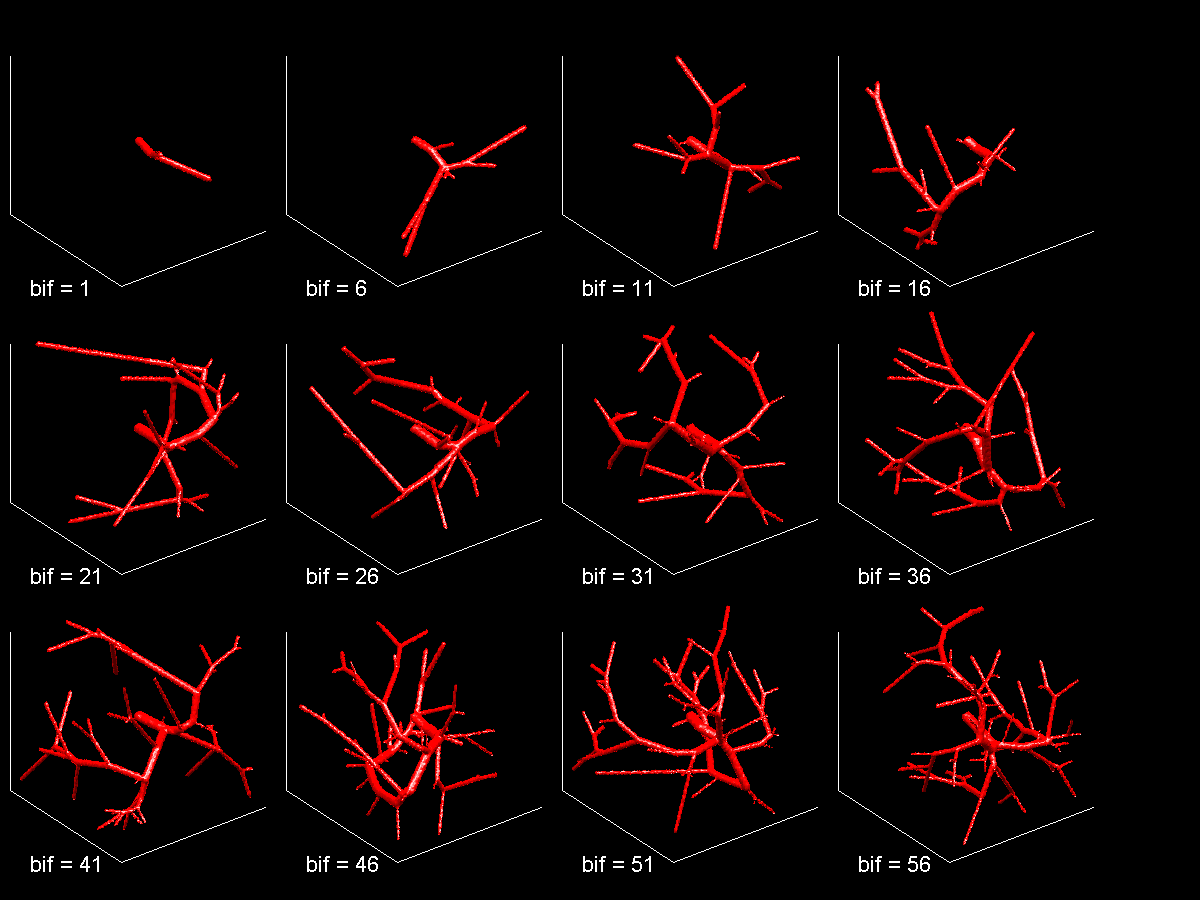
\includegraphics[height=8cm]{Images/snapVascu.png}
  
  \caption{Illustration des vaisseaux de la base VascuSynth\_2013. Le jeu de données \newV{présente une quantité variable de bifurcations.}}
  \label{fig:snap_vascu}
\end{figure}

Nous avons utilisé dans nos expériences la base de données VascuSynth\_2013, disponible sur le site de VascuSynth \footnote{\url{https://vascusynth.cs.sfu.ca/Data.html}}. VascuSynth produit des images en niveaux de gris de 0 à 255. L'intensité des vaisseaux est relativement forte : 223 pour les vaisseaux principaux avant de décroître après chaque bifurcation. L'intensité des vaisseaux décroît légèrement sur les bords de ceux-ci. On peut obtenir une vérité terrain au pixel près en binarisant ce volume initial.

La génération des artefacts IRM pour VascuSynth a connu plusieurs versions que nous détaillons ici. La version 1 a connu 4 étapes principales :
\begin{enumerate}
\item ajuster l'intensité des vaisseaux ;
\item modifier la valeur du fond constant ; 
\item ajouter des artefacts d'illumination gaussiens ;
\item ajouter du bruit.
\end{enumerate}

\subsubsection{Version 1}
\paragraph{Étapes 1 et 2}

\newV{Premièrement, l'intensité initiale des vaisseaux était trop élevée. Elle était proche de la limite maximale définie par l'encodage des images de VascuSynth (8 bits, 255 niveaux de gris). L'ajout de bruit et d'artefacts additifs n'est donc pas possible sans créer un effet de plateau d'intensités par saturation des voxels, faisant ainsi disparaître les structures. Dans l'imagerie du foie avec agent de contraste, les vaisseaux sont en principe d'intensité supérieure ou égale à l'intensité des tissus. Nous avons donc réalisé une simple mise à l'échelle des intensités avec l'intensité du fond fixée à 50 et l'intensité maximale des vaisseaux à 100 (Fig. \ref{fig:VB}).}

\begin{figure}[!ht]
  \centering
  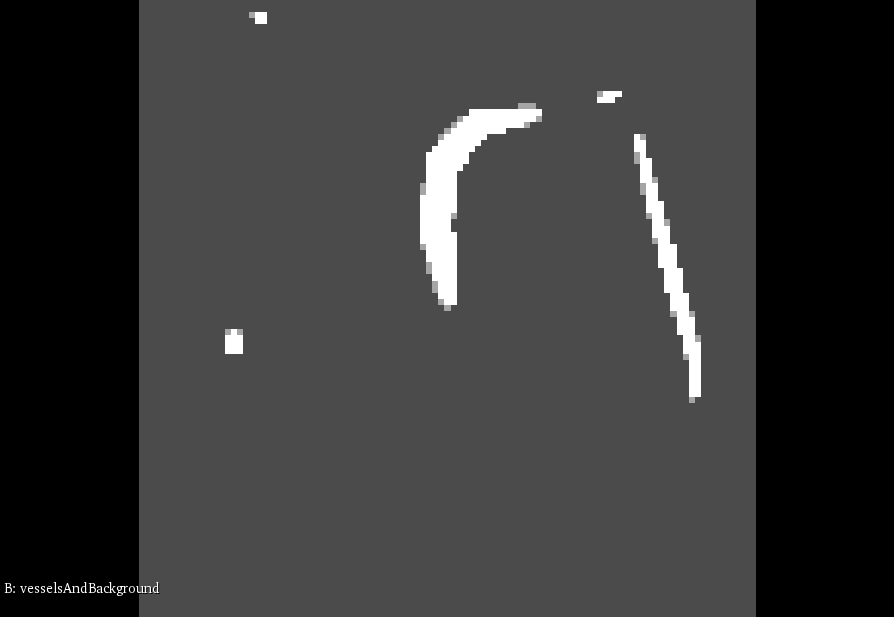
\includegraphics[height=4cm]{Images/2D_VB.png}
  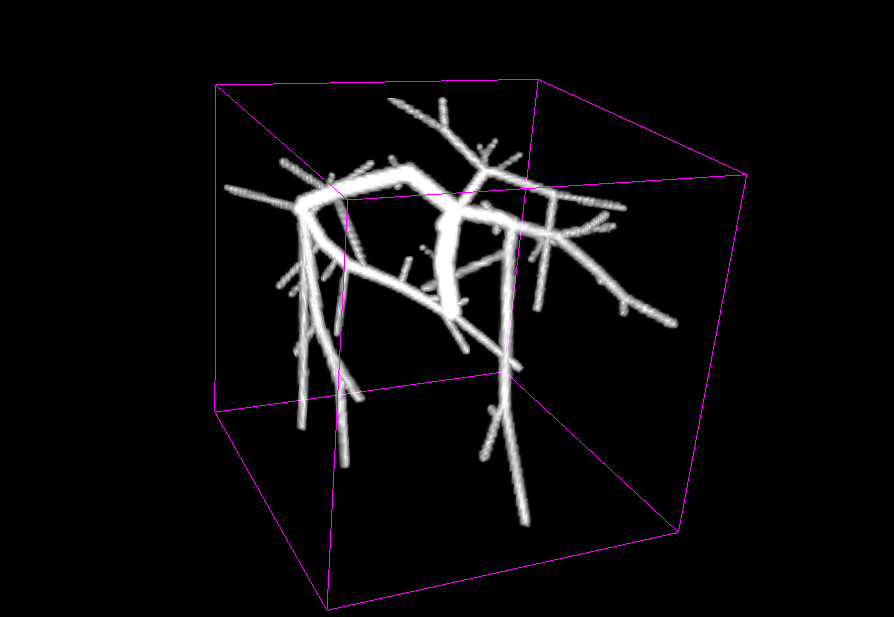
\includegraphics[height=4cm]{Images/3D_VB.png}
  
  \caption{Vue 2D (à gauche) et 3D (à droite) d'un volume original de VascuSynth auquel est rajouté un fond constant. Le fond est d'intensité égale à l'intensité minimale des vaisseaux.}
  \label{fig:VB}
\end{figure}

Pour cette première version, nous avons laissés les variations d'intensité des vaisseaux du jeu de données d'origine. \newV{Simuler des variations réalistes  d'intensité à l'intérieur des vaisseaux dépend des propriétés de mécaniques des fluides de l'agent de contraste dans le sang qui est difficile à modéliser. Nous proposons tout de même une approximation de ces variations dans une seconde version.}

\paragraph{Étape 3}

Nous avons ensuite voulu simuler les variations d'intensité locales provoquées par le positionnement du corps en fonction du champ magnétique présenté dans le chapitre \chapContextN{}. Pour cela, nous avons créé trois gaussiennes d'écart-type $\sigma=40$ pour lesquels nous avons réajusté les intensités entre 50 et 100. Le centre de ces gaussiennes sont positionnés de manière aléatoire dans le volume puis un opérateur max est appliqué entre les intensités des voxels des gaussiennes et les intensités des voxels du volume.

Cet opérateur avait été choisi dans cette première version pour simuler des vaisseaux se fondant avec l'intensité des tissus environnants (Fig. \ref{fig:VBI}). Nous sommes revenu sur ce choix dans la seconde version décrite ci-après.

\begin{figure}[!ht]
  \centering
  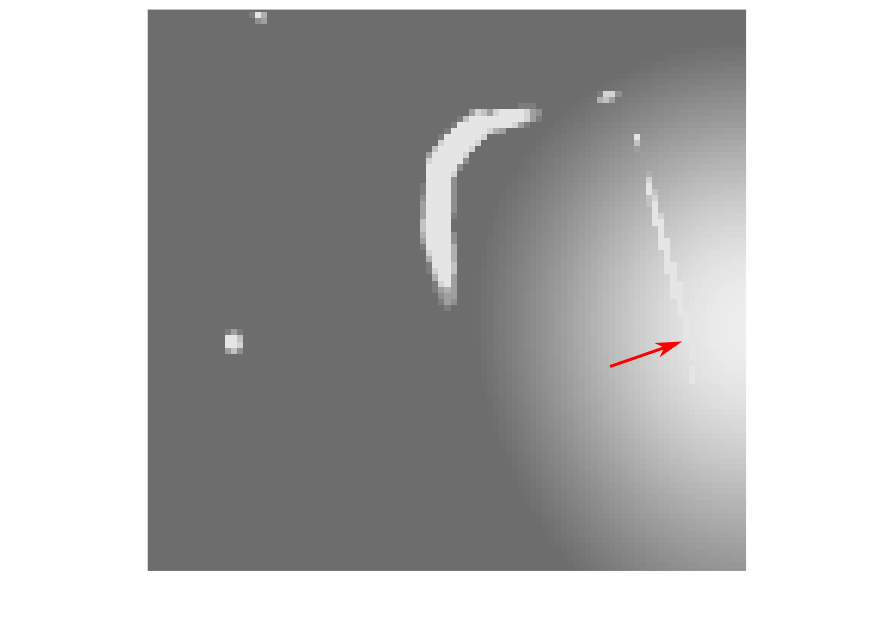
\includegraphics[height=4cm]{Images/2D_VBI.png}
  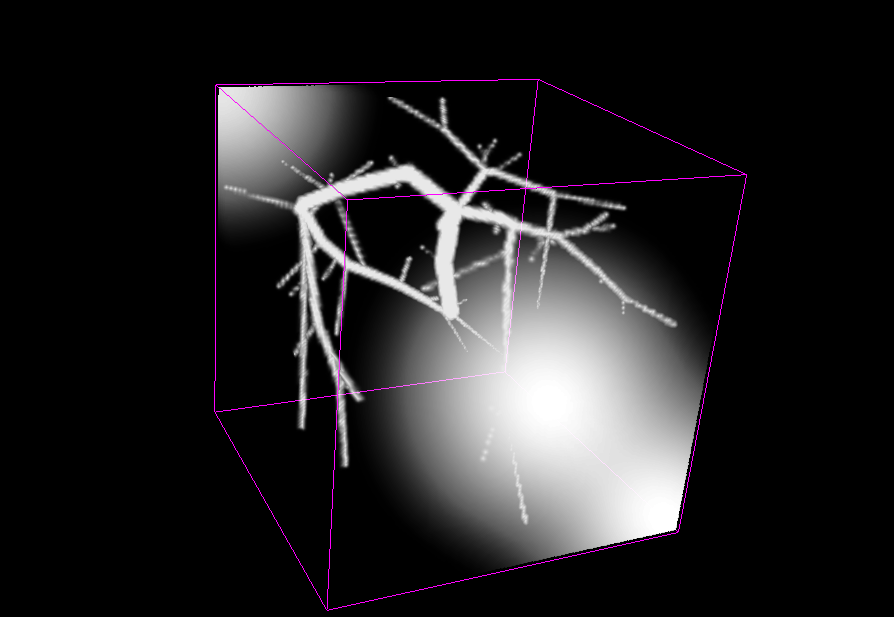
\includegraphics[height=4cm]{Images/3D_VBI.png}
  
  \caption{Vaisseaux avec illumination. Certains vaisseaux disparaissent dans les tissus.}
  \label{fig:VBI}
\end{figure}

\paragraph{Étape 4}

Nous avons ensuite ajouté du bruit ricien spécifique à l'IRM dont nous avons fait varier l'écart-type des gaussiennes qui composent la densité de probabilité. Nous avons choisi empiriquement les valeurs $\sigma=5$, $\sigma=10$ et $\sigma=20$ (Fig. \ref{fig:VBIR}). En comparaison, la plupart des expériences sur des bases de données synthétiques appliquent un mélange de bruit de Poisson et gaussien caractéristique du bruit présent en tomodensitométrie.

\begin{figure}[!ht]
  \centering
  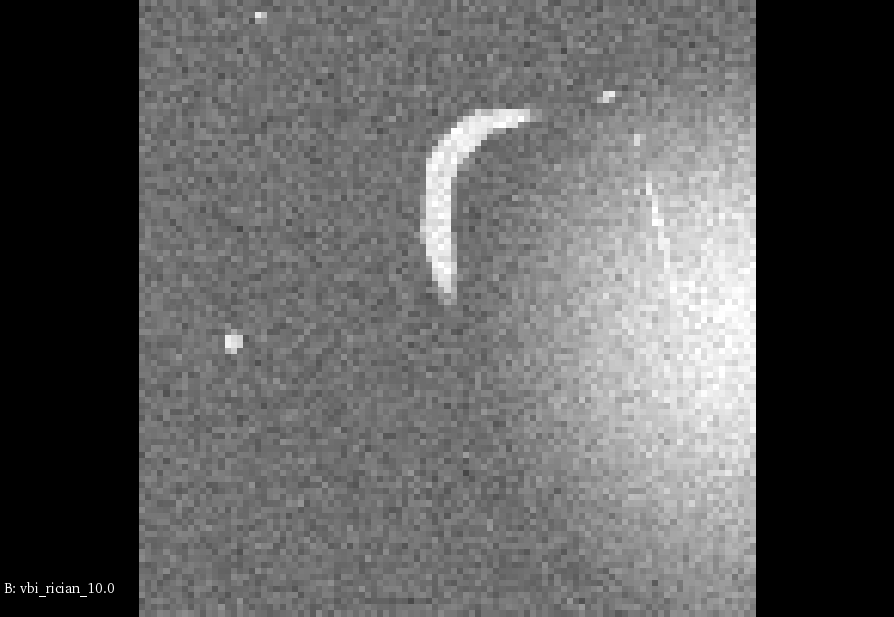
\includegraphics[height=4cm]{Images/2D_VBIR10.png}
  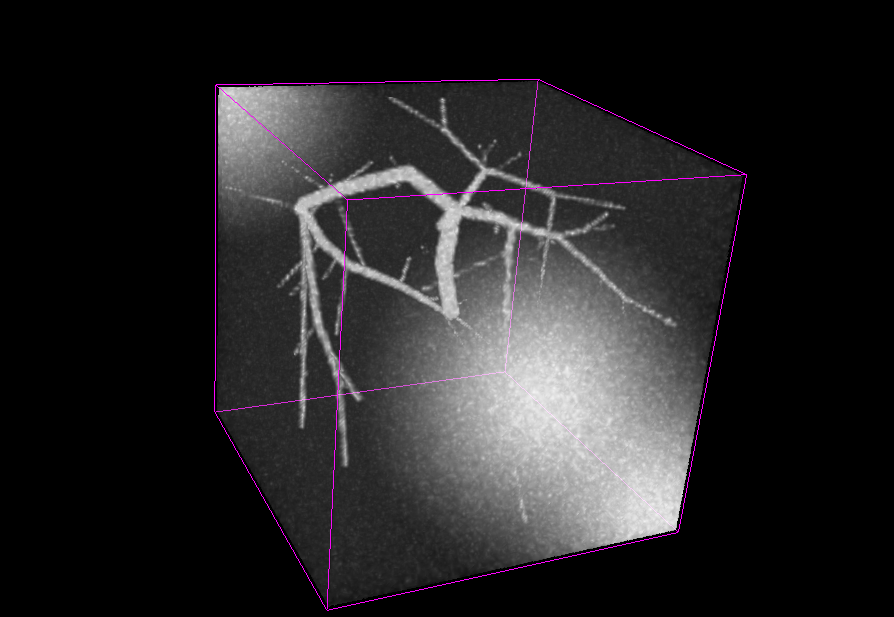
\includegraphics[height=4cm]{Images/3D_VBIR10.png}
  
  \caption{Résultat de l'étape 4 : ajout de bruit ricien sur l'image obtenue à l'étape 3 (\ref{fig:VBI}).}
  \label{fig:VBIR}
\end{figure}

\paragraph{Limitations} Cette version était une première approximation. Elle souffre cependant de plusieurs limitations. Premièrement, la dynamique d'intensité est établie de manière visuelle. Il en est de même pour l'intensité du bruit ricien. Deuxièmement, le maximum calculé entre les images et les vaisseaux fait disparaître le signal des vaisseaux qui sont tout de même présents dans la vérité terrain. On introduit ainsi une diminution artificielle des performances des filtres puisque qu'aucuns d'entre eux n'est en réalité capable de rehausser ces structures devenues invisibles. Il serait envisageable de proposer un système de reconnexion des vaisseaux pour les déconnexions importantes dans un filtre de rehaussement, mais les méthodes existantes en sont dénuées. Enfin, la plupart des vaisseaux peuvent être récupérés par un seuillage simple lorsque le niveau de bruit ne recouvre pas le signal. Ce problème est visible en MIP puisque l'intégralité des vaisseaux sont visibles quand ils ne sont pas recouverts par des blobs gaussiens (voir Fig. \ref{fig:vascu_v1_problems}).

\begin{figure}[!ht]
  \centering
  \begin{subfigure}{0.45\textwidth}
    \centering
    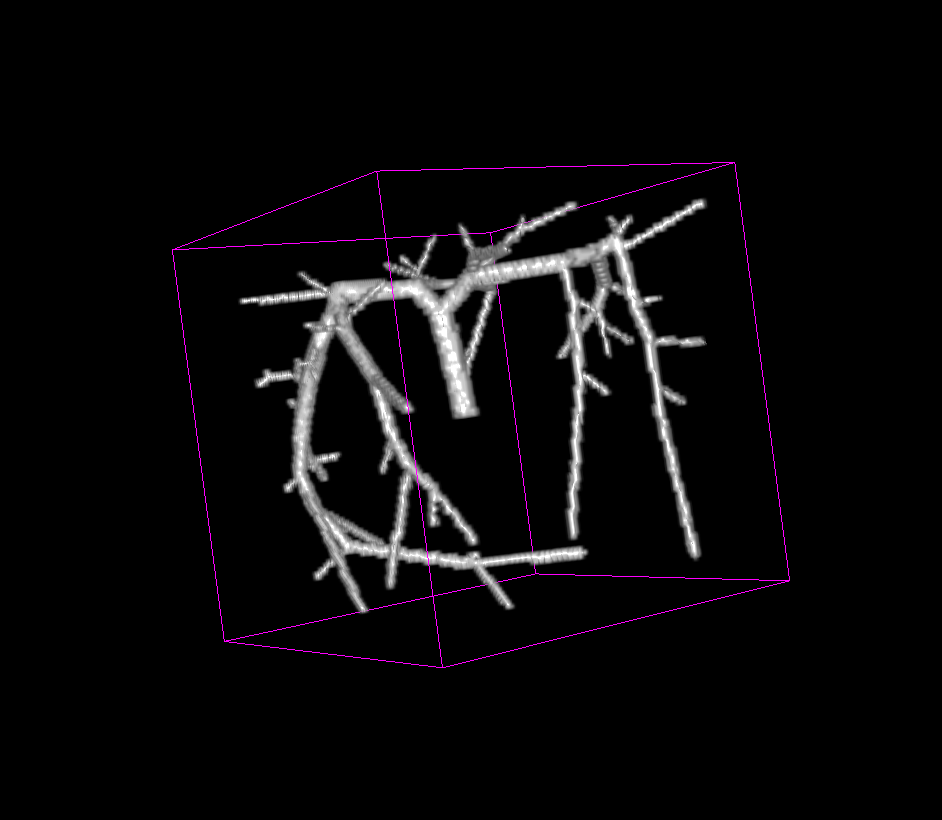
\includegraphics[width=\textwidth]{Images/vascu_v1_gt.png}
    \caption{Vérité terrain}
  \end{subfigure}
  \begin{subfigure}{0.45\textwidth}
    \centering
    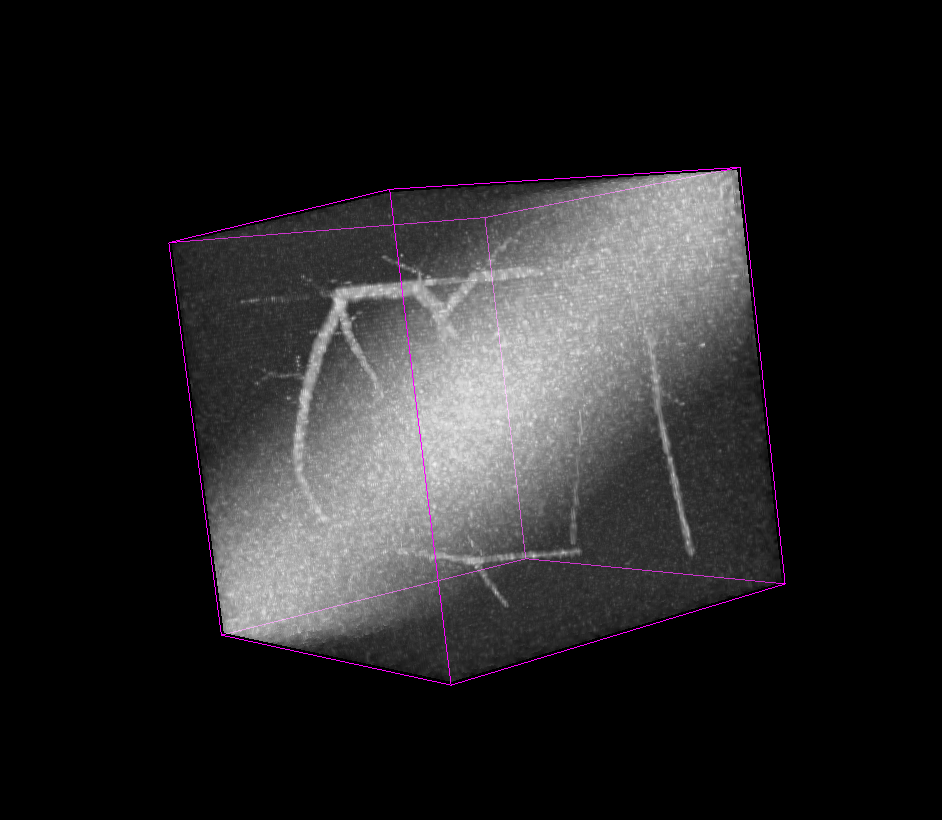
\includegraphics[width=\textwidth]{Images/vascu_v1_original.png}
    \caption{Volume IRM simulé (MIP)}
  \end{subfigure}
  \begin{subfigure}{0.45\textwidth}
    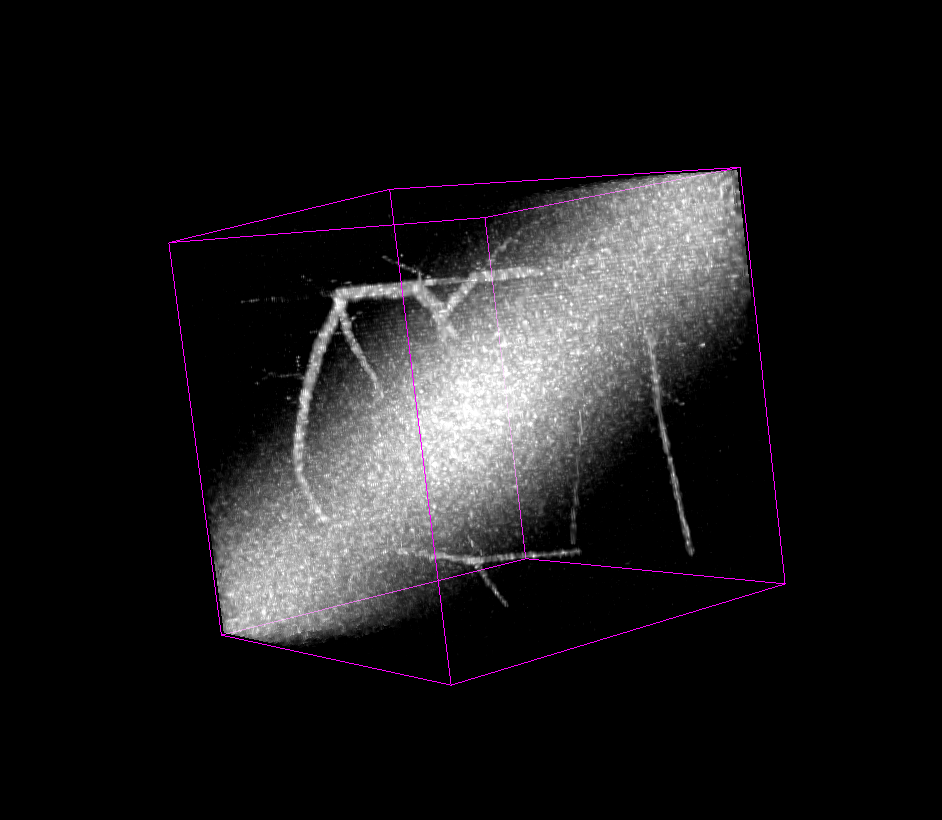
\includegraphics[width=\textwidth]{Images/vascu_v1_thresholding.png}
    \centering
    \caption{Volume seuillé (MIP)}
  \end{subfigure}
  \caption{Vérité terrain et projection d'intensités maximales (MIP) d'une image générée avec la première version. La majeure partie des vaisseaux peut être obtenue par simple seuillage lorsque ceux-ci ne sont pas perdus dans les artefacts d'illumination.}

  \label{fig:vascu_v1_problems}
\end{figure}

\subsubsection{Version 2}

Dans une deuxième itération, nous avons revu le processus de création de ces volumes. Premièrement, les volumes ont été redimensionnés par ajout de zéros (padding) pour que leur taille passe de $101 \times 101 \times 101$ à $128 \times 128 \times 128$ voxels. Ce changement nous a permis de faciliter l'utilisation de cette base synthétique avec des méthodes de deep learning (Chap. \ref{sec:Ending}).

\paragraph{Étapes 1 et 2}
Comme pour la version 1, un fond constant égal à l'intensité minimale des vaisseaux est ajouté. De même, l'intensité des vaisseaux est aussi réajustée. Cette fois ci, la plage d'intensité des vaisseaux est définie à partir de mesures de l'intensité des voxels issue d'IRM réelles de foie. Ces mesures ont été réalisées manuellement sur 5 volumes issus du projet R-Vessel-X. Pour chaque volume, nous avons annoté 3 coupes relativement espacés à l'intérieur du foie.Pour chaque coupe, nous avons annoté manuellement le fond et les vaisseaux afin d'obtenir un histogramme de la répartition des intensités pour les tissus et les vaisseaux par volume. Pour chaque volume, nous avons adapté une distribution gaussienne aux données (Fig. \ref{fig:Distributions_mri_intensities}),  puis nous avons moyenné les courbes de manière à obtenir une distribution moyenne (Fig. \ref{fig:Distributions_mri_mean}).

\begin{figure}[!ht]
  \centering
  \begin{subfigure}{\textwidth}
    \centering
    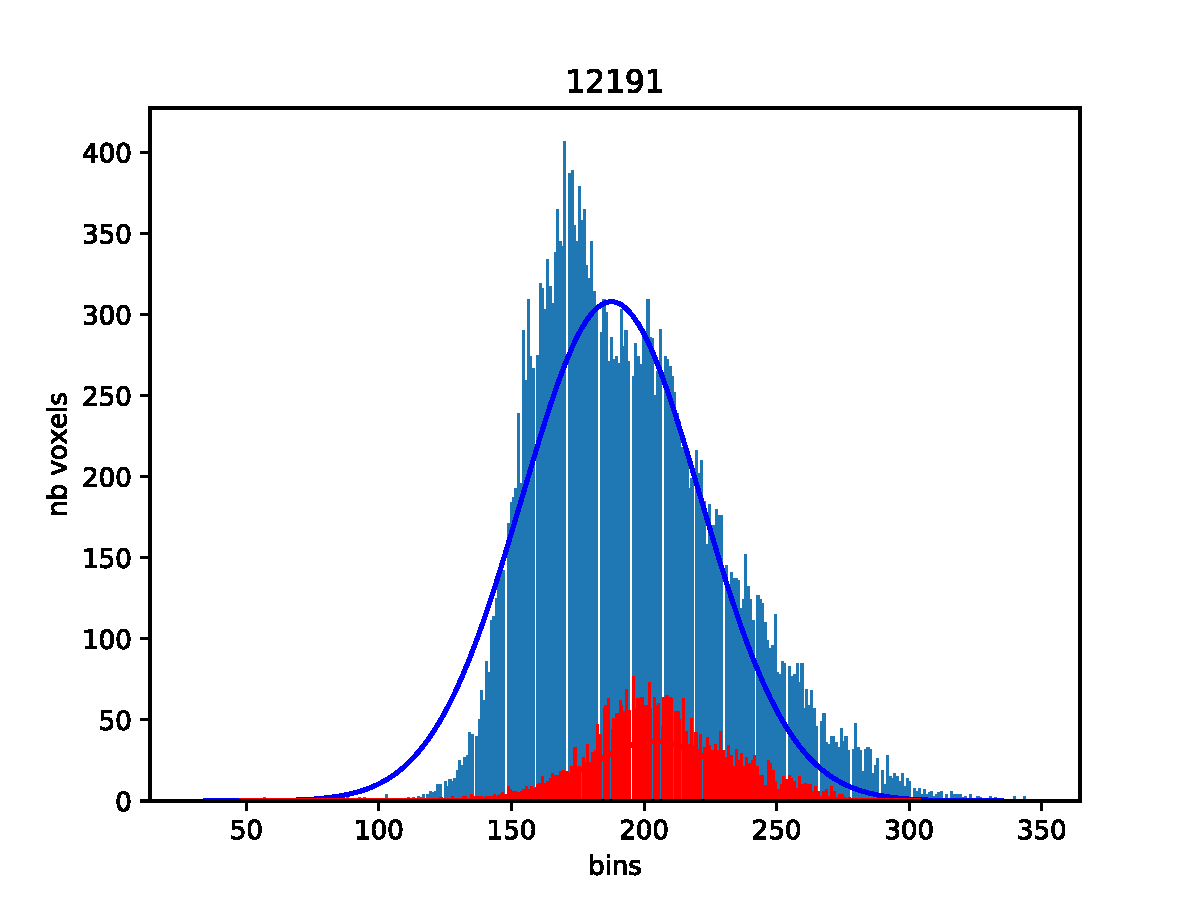
\includegraphics[height=4cm]{Images/gen_12191.pdf}
    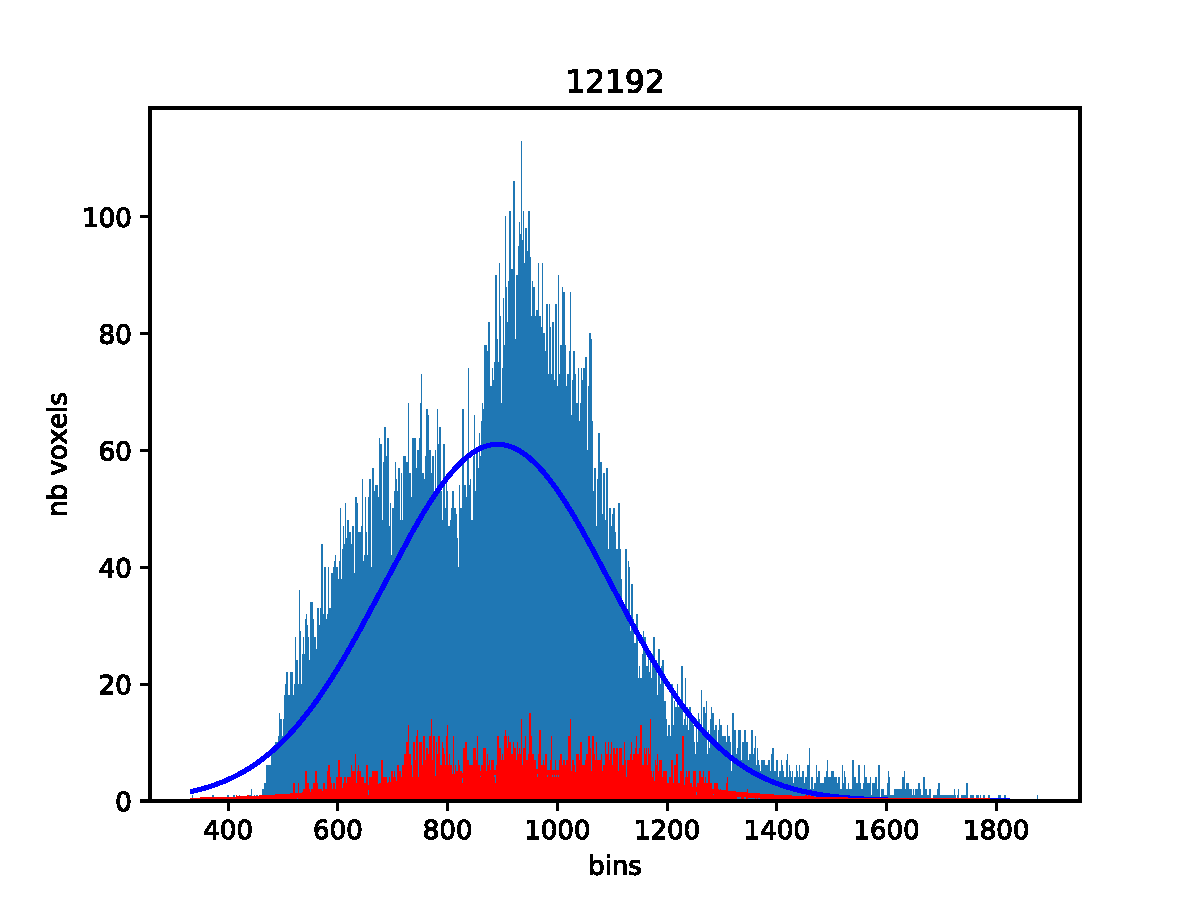
\includegraphics[height=4cm]{Images/gen_12192.pdf}
    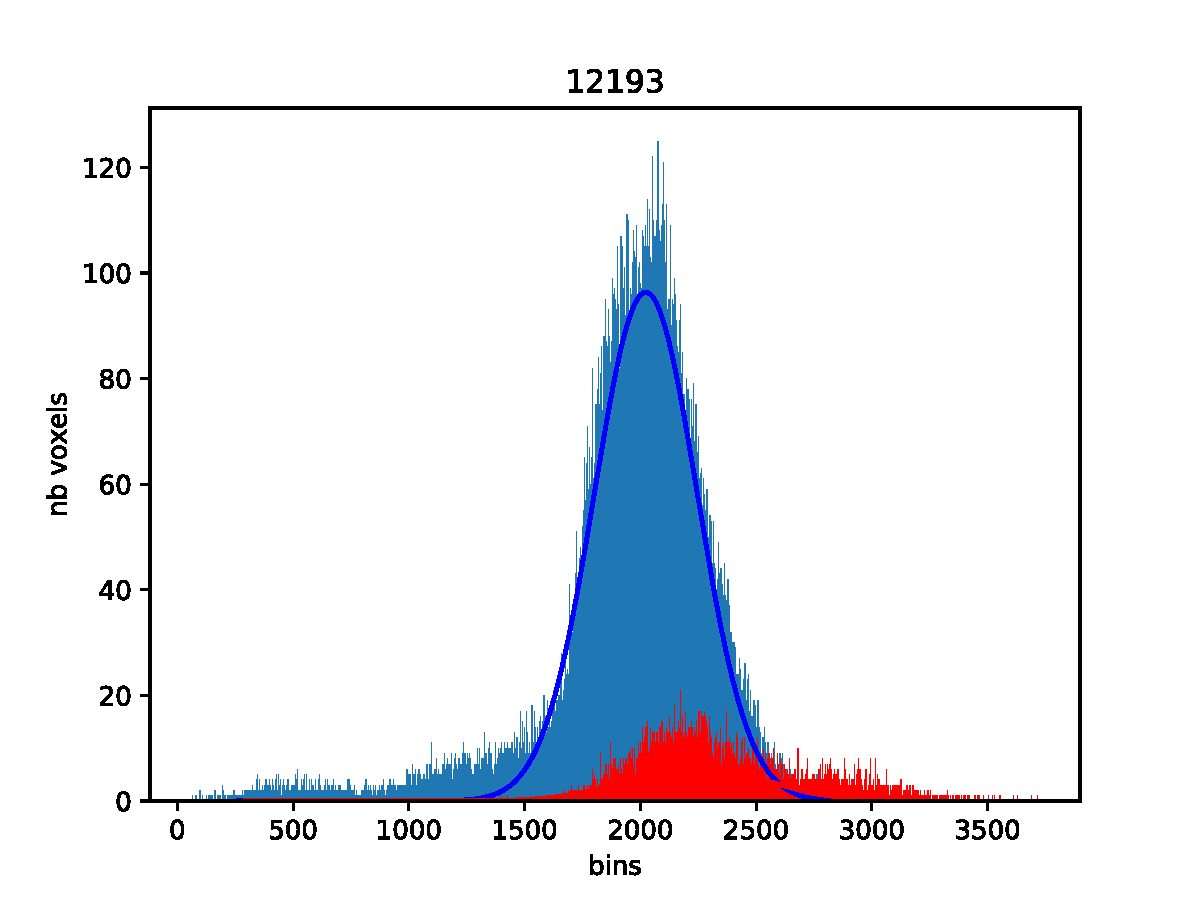
\includegraphics[height=4cm]{Images/gen_12193.pdf}
    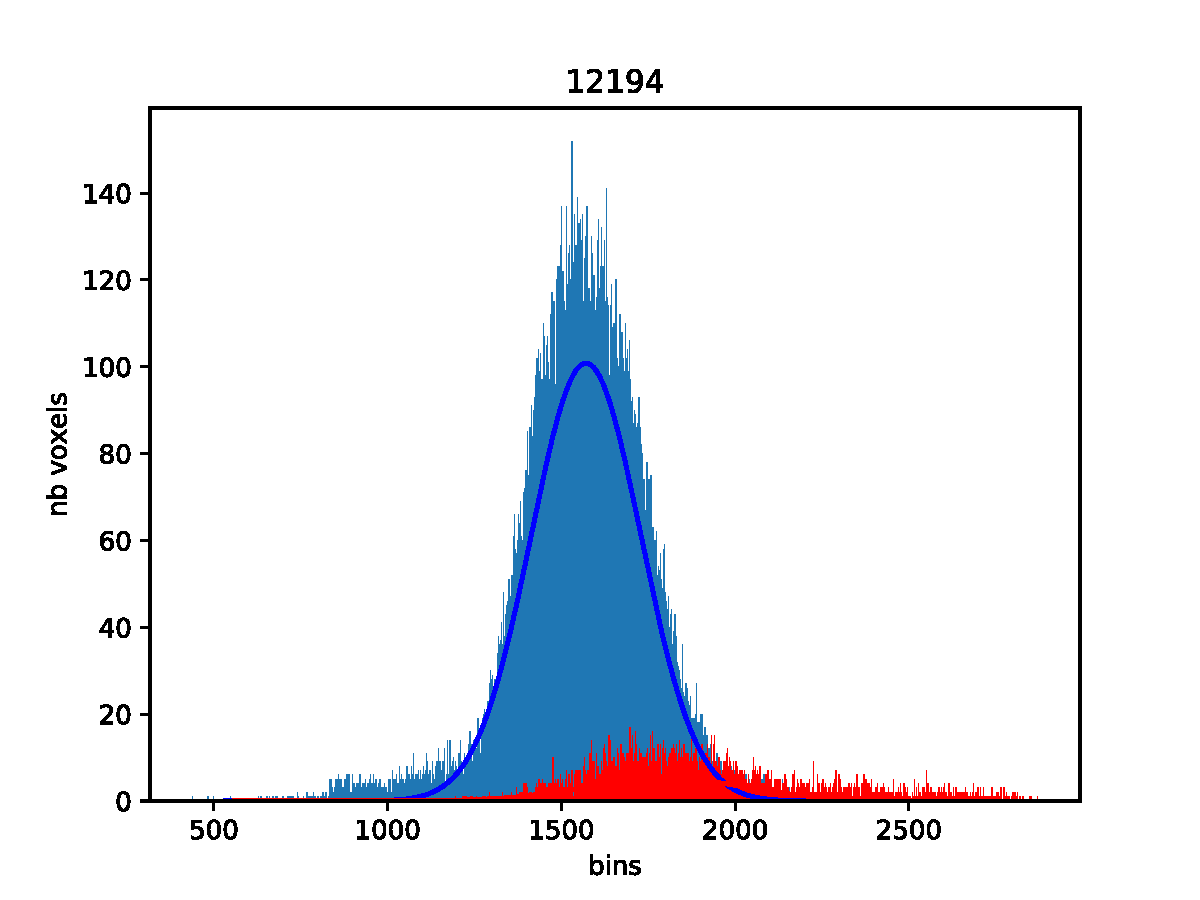
\includegraphics[height=4cm]{Images/gen_12194.pdf}
    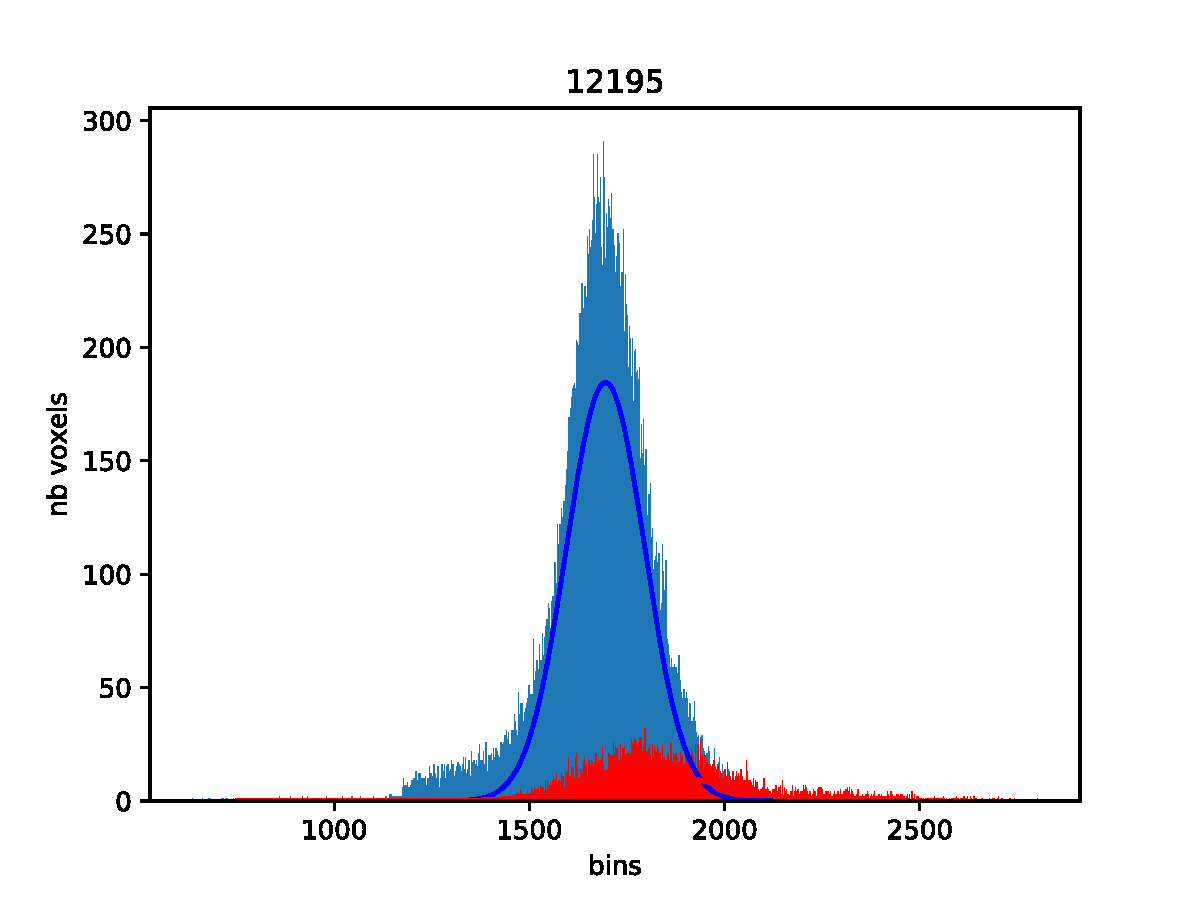
\includegraphics[height=4cm]{Images/gen_12195.pdf}
  \end{subfigure}
  \caption{Histogramme des intensité des volumes IRM du foie (anonymisés) ayant servis à modéliser les intensités moyennes des voxels pour VascuSynth. Des modèles gaussien représenté par les courbes rouges et bleu a été extrait pour chacune des distributions. Les voxels appartenant aux vaisseaux apparaissent en rouge et les autres en bleu. On note que les intensités des vaisseaux sont inclus dans l'intervalle d'intensité des tissues du foie.}
  \label{fig:Distributions_mri_intensities}
\end{figure}
\begin{figure}[!ht]
  \begin{subfigure}{\textwidth}
    \centering
    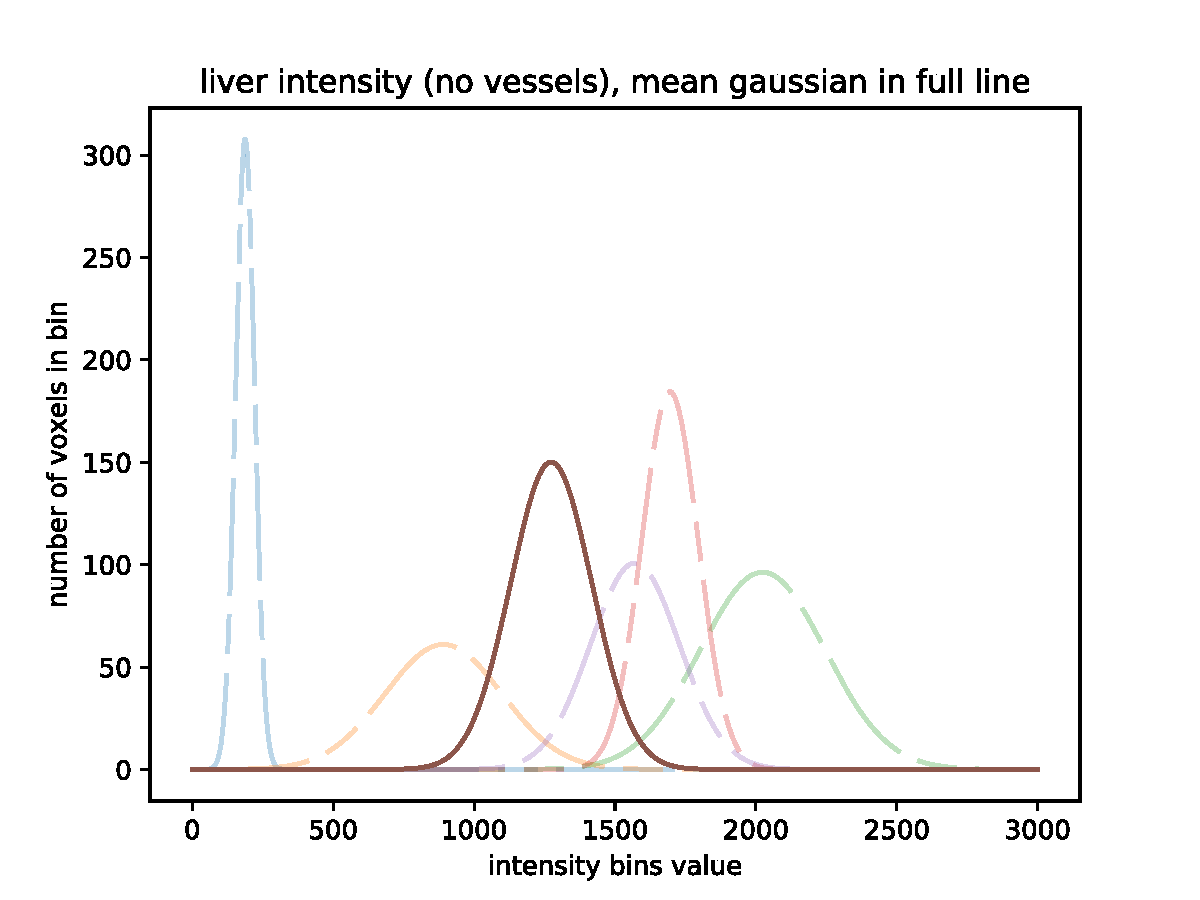
\includegraphics[width=0.45\textwidth]{Images/gen_mri_liver_mean_intensity.pdf}
    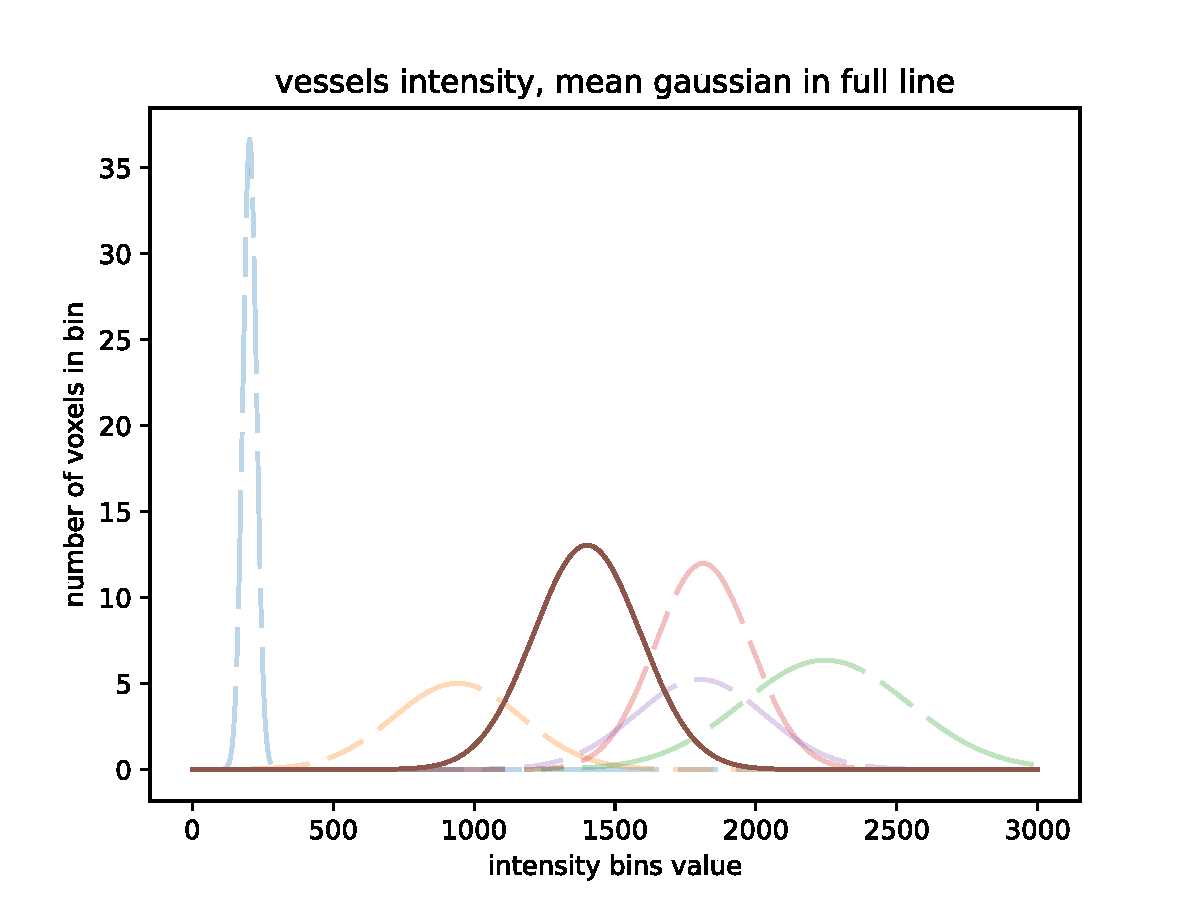
\includegraphics[width=0.45\textwidth]{Images/gen_mri_vessels_mean_intensity.pdf}
    
  \end{subfigure}
  \caption{Distribution moyenne pour les tissus du foie (gauche) et les vaisseaux (droite). La distribution moyenne de l'ensemble des distributions des volumes est affichée en traits pleins.}
  \label{fig:Distributions_mri_mean}
\end{figure}

Ainsi, pour des voxels d'images IRM compris dans l'intervalle $[0,3000]$ la moyenne de l'intensité des tissus du foie hors vaisseaux est de $1273 \pm 144$ et celle des vaisseaux $1400 \pm 189$. Ramené à une dynamique d'intensité comprise entre $[0, 255]$ on obtient $108 \pm 12$ pour les tissus hors vaisseaux et $119 \pm 16$ pour les vaisseaux. \newV{L'écart entre la moyenne des intensités des tissus et celle des vaisseaux est faible. En pratique, cet écart est plus élevé localement. Nous avons donc considéré l'intensité des vaisseaux comme la somme de leur moyenne et de leur écart-type. On peut ainsi augmenter la dynamique de niveau de gris tout en restant cohérent avec les mesures physiques. Une trop petite dynamique dégrade aussi le profil des gaussiennes utilisées dans les étapes suivant en formant une pente crénelée plutôt que lisse. Augmenter l'interval d'intensité donne aux gaussiennes un profil décroissant plus régulier.}

\paragraph{Étape 3}

\newV{Dans cette version, nous avons introduit deux types supplémentaires de variations d'intensités via deux filtres : un premier pour faire varier le profil d'intensité des vaisseaux et un second pour faire varier l'intensité globale de l'image. Dans le premier cas, celle-ci essaie d'approcher les variations d'intensités liées à l'agent de contraste. Dans le second cas, cette modification a été faite pour que le jeu de données soit résistant à une segmentation par simple seuillage.} L'objectif est alors que localement les vaisseaux restent des maxima locaux, mais que ceux-ci soient d'intensité plus faible que des tissus du foie situés à l'autre extrémité du volume.

Pour inclure ces améliorations, l'algorithme de génération change légèrement. Pour le changement d'intensité dans les vaisseaux, on utilise un masque avec des gaussiennes tirées aléatoirement ; ces gaussiennes sont pondérées de manière à faire diminuer l'intensité des vaisseaux au maximum de $30$ \percent{} par rapport à leur intensité initiale. Les gaussiennes étant tirées dans l'espace entier de l'image on obtient des variations non linéaires le long des vaisseaux.

La pondération de l'ensemble de l'image par des gaussiennes est effectuée pour que la diminution d'intensité atteigne au maximum $40$ \percent{} de l'intensité originale des pixels.

Des artefacts gaussiens sont ajoutés pour venir perturber les filtres de rehaussement en introduisant des structures faiblement tubulaires, planaires ou en forme de blob. Pour cela, une dizaine d'éléments gaussiens sont introduits avec un sigma aléatoire pour chaque axe de l'image. Ces artefacts sont introduits de manière additive. Par conséquent, cette opération ne provoque aucune disparition de vaisseaux. Dans le pire des cas, un saut d'intensité est observé.

\paragraph{Étape 4}
Enfin, le bruit ricien est ajouté. L'écart d'intensité entre le fond et les vaisseaux étant plus faible sur cette version, nous avons revu les différents niveaux de bruits appliqués aux volumes tel que $\sigma={2,4,6}$.

Les étapes de génération des volumes pour cette version sont :

\begin{enumerate}
  \item ajuster l'intensité des vaisseaux ;
  \item pondérer l'intensité des vaisseaux par des gausiennes ;
  \item ajouter un fond constant ; 
  \item pondérer l'intensité de l'ensemble de l'image par des gaussiennes ;
  \item ajouter des artefacts intenses gaussiens ;
  \item ajouter du bruit.
  \end{enumerate}

En conclusion, nous générons 360 volumes (120 volumes pour chaque niveau de bruit) contenants un arbre vasculaire et 4 types d'artefacts courants dans les images d'IRM (Fig. \ref{fig:vascuSynth_results_V2}).

\begin{figure}
\captionsetup[subfigure]{justification=centering}

\begin{subfigure}{\textwidth}
  \centering
  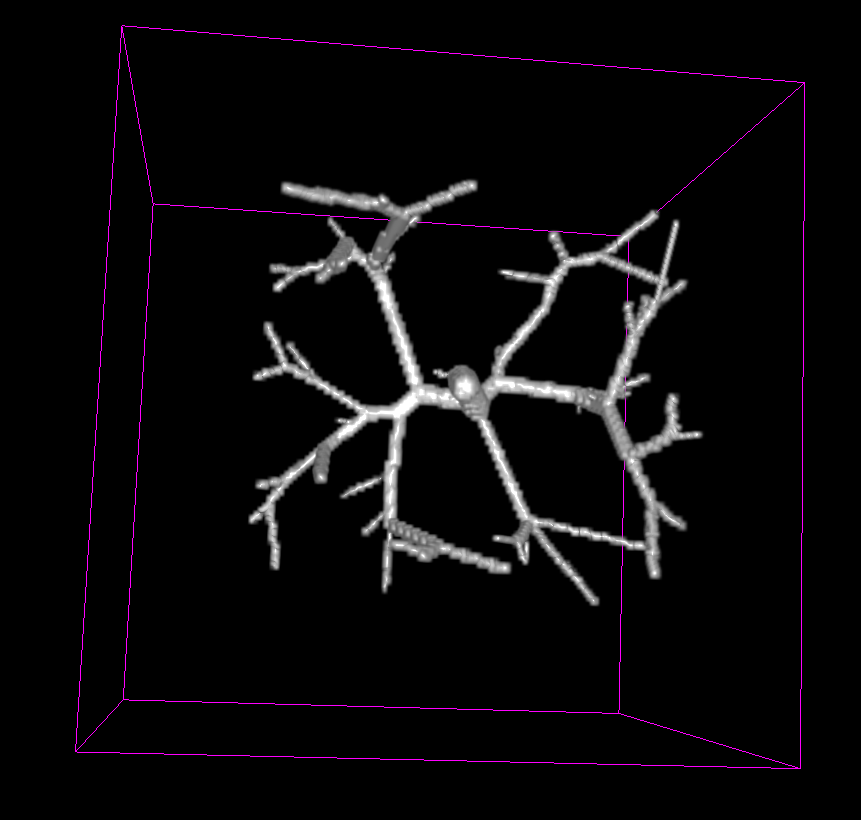
\includegraphics[height=6cm]{Images/gen_vascu_V2_GT.png}
  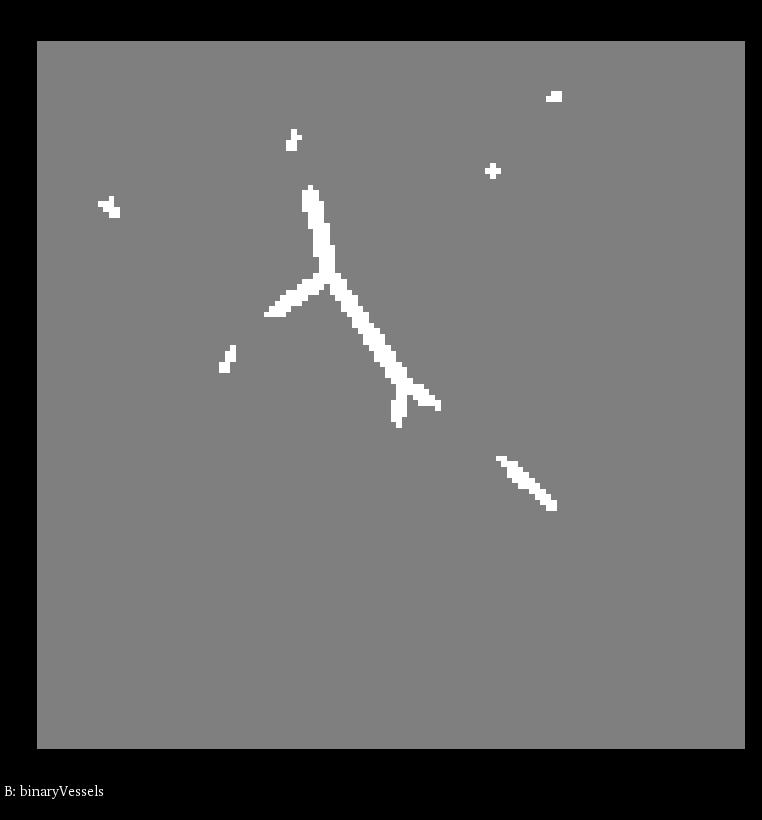
\includegraphics[height=6cm]{Images/gen_vascu_V2_GT_2D.png}
  \caption{Vérité terrain}
\end{subfigure}
\begin{subfigure}{\textwidth}
  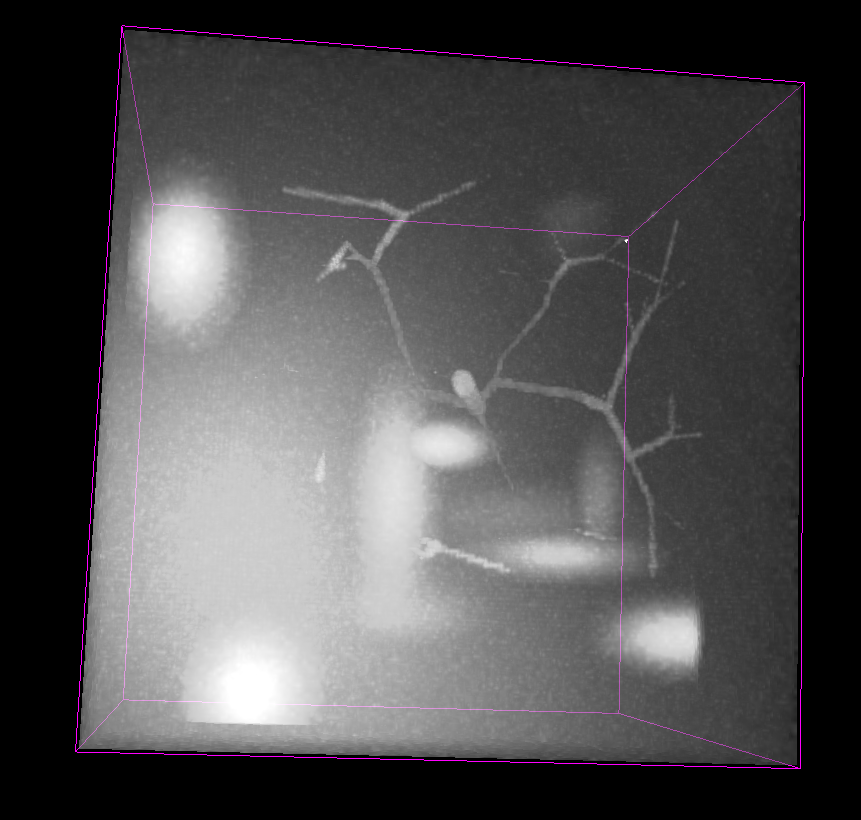
\includegraphics[width=0.32\textwidth]{Images/gen_vascu_V2_r2.png}
  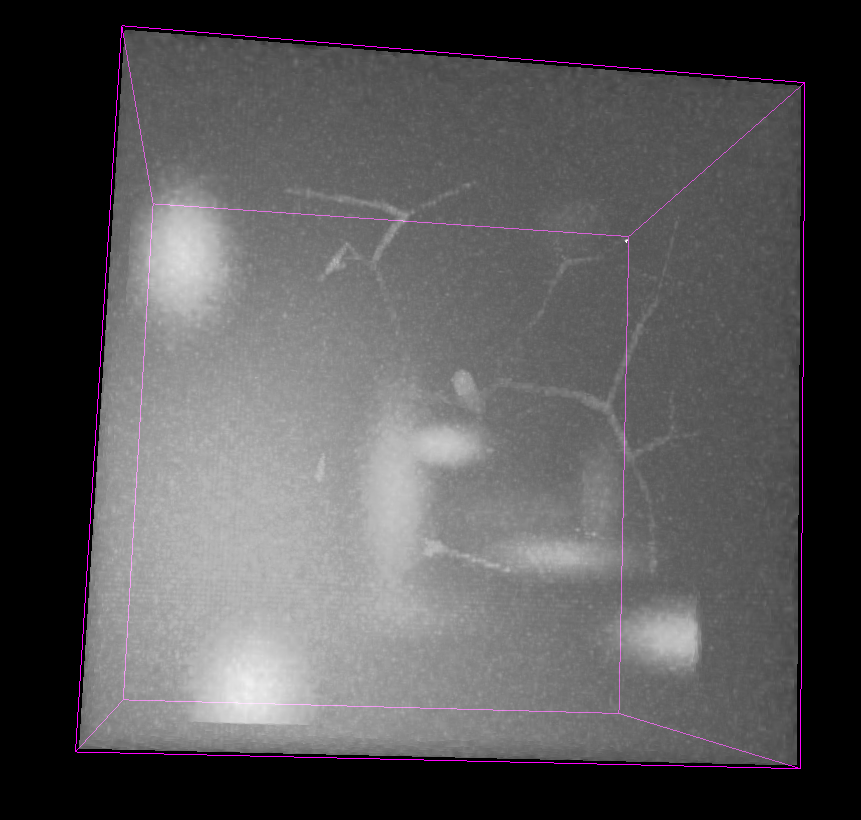
\includegraphics[width=0.32\textwidth]{Images/gen_vascu_V2_r4.png}
  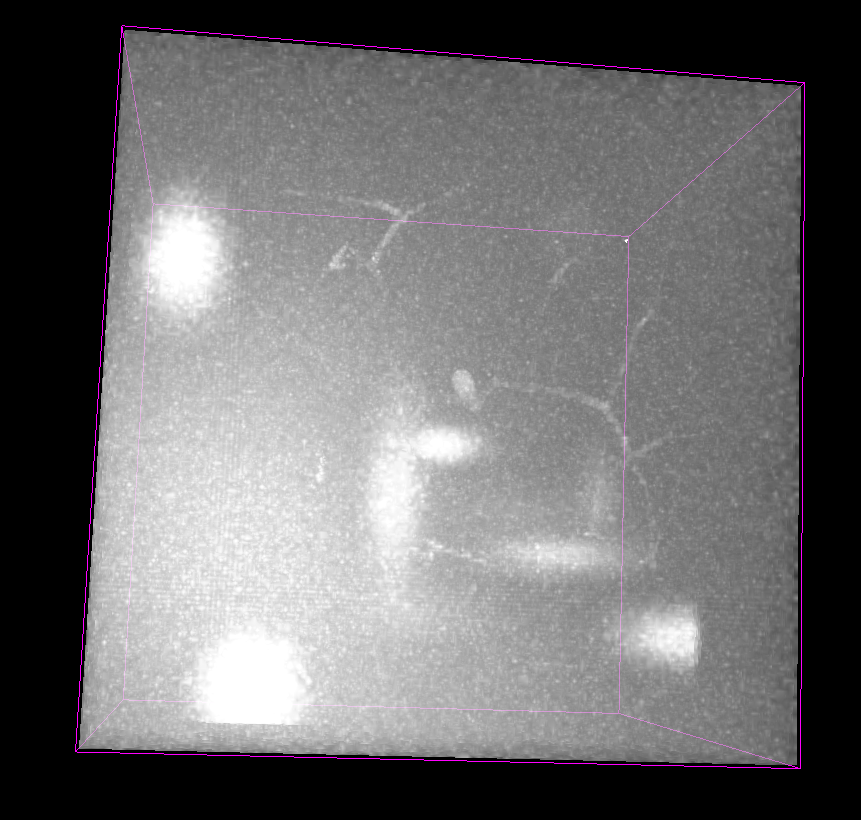
\includegraphics[width=0.32\textwidth]{Images/gen_vascu_V2_r6.png}
  \caption{Volumes 3D générés avec un bruit ricien croissant $\sigma=\{2, 4, 6\}$.}
\end{subfigure}
\begin{subfigure}{\textwidth}
  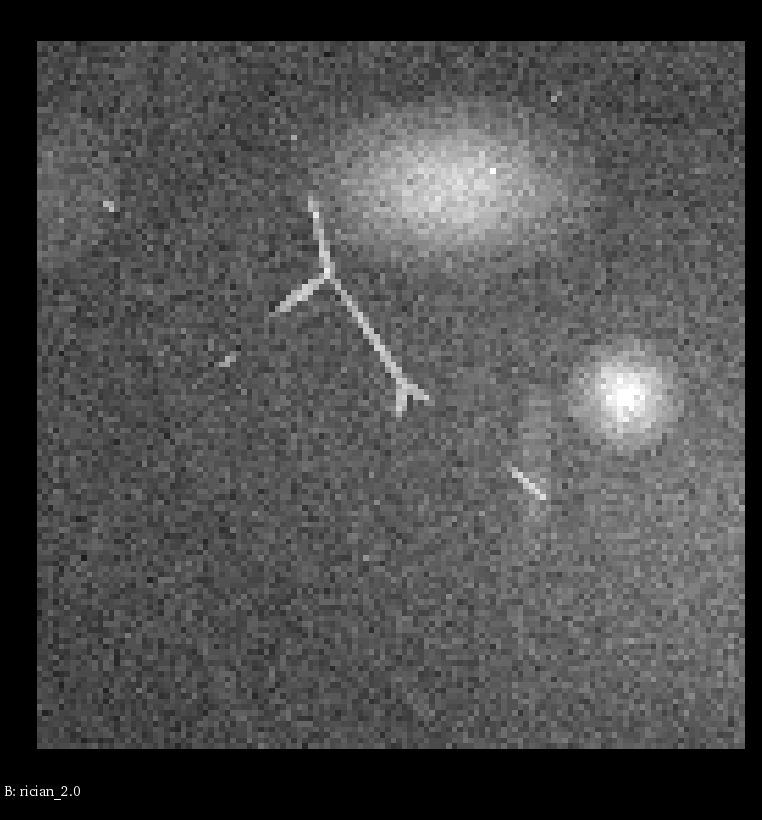
\includegraphics[width=0.32\textwidth]{Images/gen_vascu_V2_r2_2D.png}
  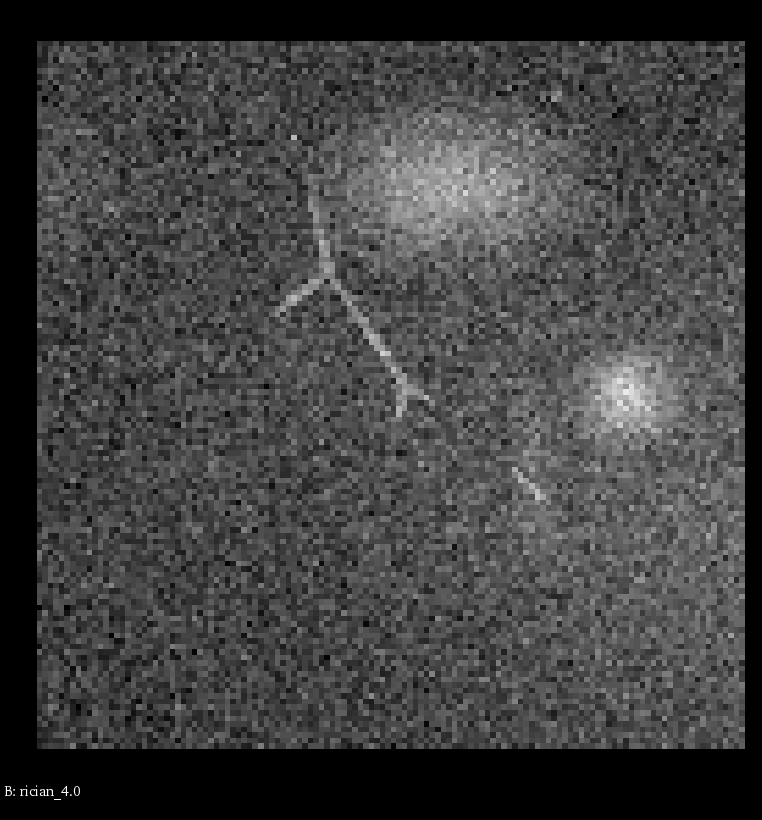
\includegraphics[width=0.32\textwidth]{Images/gen_vascu_V2_r4_2D.png}
  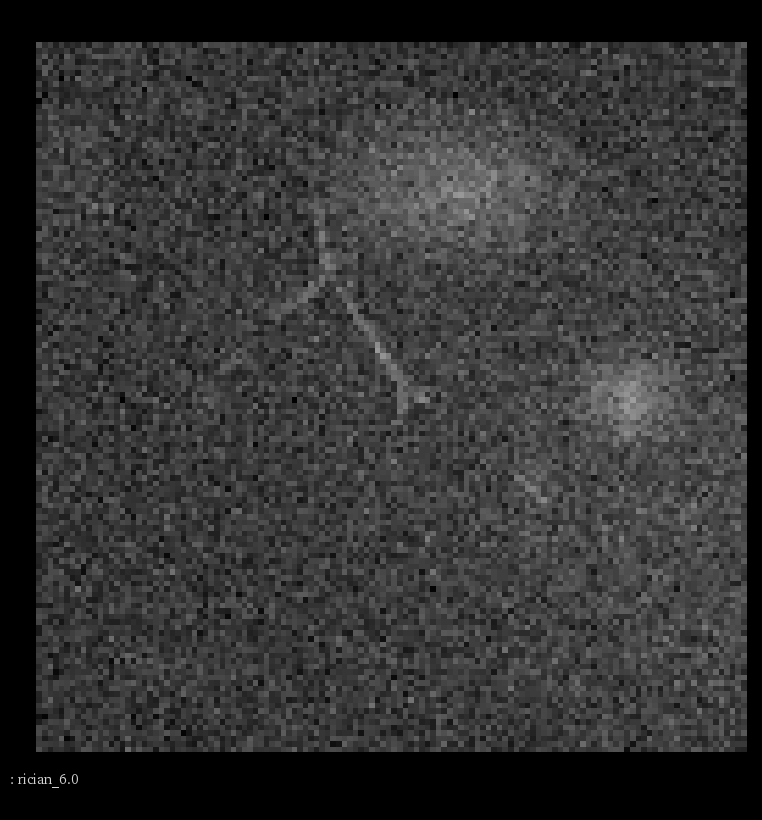
\includegraphics[width=0.32\textwidth]{Images/gen_vascu_V2_r6_2D.png}
  \caption{Coupes des volumes 3D avec un bruit ricien croissant $\sigma=\{2, 4, 6\}$.}
\end{subfigure}
\caption{Illustration des volumes générés avec la seconde version de simulation d'artefacts IRM. Les vaisseaux restent localement visibles malgré un contexte global complexe.}
\label{fig:vascuSynth_results_V2}
\end{figure}
 
\section{Construction des zones d'évaluation des filtres}
\label{sec:evaluation}
\newV{De manière générale on évalue un algorithme dans le voisinage global de l'organe que l'on traite. Par exemple, lorsque l'on veut segmenter le cerveau, on évalue la performance de la segmentation sur l'image globale. Pour les vaisseaux, on évalue généralement un traitement par rapport à l'organe correspondant : le foie pour l'Ircad ou le cerveau pour Bullit.}

\newV{Cette évaluation globale n'est cependant pas suffisante seule pour évaluer le rehaussement de manière précise, puisqu'un filtre peut se comporter différemment en fonction des structures présentes localement. Nous avons donc souhaité définir des régions d'évaluations distinctes, que nous appelons zones d'intérêt (ZI), de manière à évaluer quantitativement le rehaussement, régions 
par régions. Nous listons ici les ZI que nous avons sélectionnées et nous récapitulons leurs avantages.}

\newV{La première zone d'intérêt est \tbf{le volume de l'organe}. Comme rappelé précédemment, c'est la zone d'évaluation classique qui permet de juger des performances globales d'un filtre. Elle permet d'évaluer le rehaussement de la totalité du réseau vasculaire, mais aussi d'analyser la capacité d'un filtre à éviter les artefacts globaux comme le bruit ou les structures non tubulaires. Pour les jeux de données que nous utilisons ces structures correspondent par exemple aux tumeurs qui touchent les foies de l'Ircad, aux replis du cerveau pour Bullitt ou aux artefacts gaussien pour VascuSynth.}

La seconde région d'intérêt concerne \tbf{les vaisseaux et leur voisinage proche}. Le voisinage est défini par un ensemble de voxels dont la distance aux vaisseaux est relativement faible. Étudier le rehaussement sur les vaisseaux seuls est important. En effet, un filtre qui n'arriverait pas à filtrer les artefacts ou le bruit peut toutefois présenter un rehaussement des vaisseaux de bonne qualité. Comme notre vérité terrain est voxélique, il est plus pertinent d'étudier les voxels appartenant aux vaisseaux et à un voisinage. En effet, ajouter le voisinage permet d'inclure l'enveloppe extérieure des vaisseaux dans l'analyse et de savoir si le rehaussement surestime la taille des vaisseaux. Cette région peut être subdivisée en partitions en fonction de la taille ou de la hiérarchie des vaisseaux. On peut ainsi analyser quels types de vaisseaux, larges ou fins, sont les mieux rehaussés et dans quel contexte.

La troisième région d'intérêt concerne \tbf{les bifurcations des vaisseaux}. Cette zone est singulière, car elle correspond à une jonction des vaisseaux tubulaires. Dans cette zone, la géométrie n'est plus tubulaire et le rehaussement peut donc y être affaibli. Cette perte de signal a été signalée dans de nombreuses publications et est souvent illustrée de manière visuelle sur des données synthétiques. Par contre, elle n'a, à notre connaissance, jamais été évaluée quantitativement.

% M global
Pour la zone d'intérêt des organes, celle-ci est relativement simple à obtenir à l'aide d'outils semi-automatiques comme les level sets ou la croissance de région à partir de marqueurs placés à la main. La géométrie de la bordure des organes est la plupart du temps, simple et bien définie. Il peut cependant arriver que le mouvement du patient durant l'acquisition fasse fusionner des tissus, comme c'est souvent le cas entre le foie et l'estomac. Dans ce cas, une correction manuelle peut être nécessaire.

% M vaisseaux
La construction des zones d'intérêt du voisinage des vaisseaux passe par l'utilisation des vérités terrains.
Pour la vérité terrain des vaisseaux, une première approximation peut être obtenue par seuillage en profitant du profil d'intensité élevé des vaisseaux. Cependant, la majeure partie des annotations doit être réalisée manuellement par un expert. La création de ces vérités terrains prend du temps. \newV{À titre d'exemple, il faut environ une heure pour segmenter les vaisseaux d'une image IRM de foie.} Une paire de vues 2D et MIP 3D permet de valider les annotations de manière simple et améliore considérablement la qualité des annotations.

% M vaisseaux G - M - P
\newV{Pour obtenir une zone d'intérêt du voisinage des vaisseaux, on peut dilater la vérité terrain des vaisseaux. Nous avons dans un premier temps réalisé une dilatation globale. Cette dilatation construit un voisinage de taille constante autour des vaisseaux malgré des variations de tailles des vaisseaux. Le rapport entre le nombre de voxels du fond et des vaisseaux est donc différent pour les gros vaisseaux et les petits vaisseaux. Afin d'équilibrer ce rapport et d'observer le rehaussement en fonction de la taille des vaisseaux, nous avons séparé le voisinage des vaisseaux en trois classes pour l'Ircad et VascuSynth et deux classes pour Bullitt. Pour les deux premiers jeux de données, la première classe comprend les gros vaisseaux correspondants aux tronc des réseaux vasculaire. Une seconde classe comprend les vaisseaux de taille moyenne après les premiers embranchements et une troisième classe regroupe les petits vaisseaux des extrémités des réseaux vasculaires. Pour Bullitt, les vaisseaux présentent moins de variations de tailles et seul deux classes sont utilisés : Une classe de talles moyennes correspondant aux artères principalement localisées dans le cercle de Willis et une classe pour le reste des vaisseaux plus petits. La répartition des vaisseaux entre chaque classe nécessite de labelliser chaque branche de vaisseaux de la vérité terrain en fonction de son diamètre.}

Afin de simplifier la dénomination des masques dans le reste de ce manuscrit, nous introduisons les notations suivantes :

\begin{itemize}
  \item \maskglobal pour le masque global, qui correspond à l'organe du volume traité. (Le foie pour le jeu de l'Ircad, le cerveau pour le jeu Bullitt et l'image entière pour le jeu VascuSynth) ;
  \item \maskvascular pour le voisinage des vaisseaux, qui correspond à l'union des vaisseaux et des zones proches des vaisseaux (voir la méthode de construction ci-dessous) ;
  \item \maskvesselLarge, \maskvesselMedium, \maskvesselSmall, les masques de voisinage des vaisseaux, qui constituent une partition dépendante de la taille des vaisseaux de \maskvascular;
  \item \maskbif, le masque des bifurcations à l'intérieur des vaisseaux.
  \end{itemize}

\subsection{Masques globaux}

Nous décrivons ici la création des masques par base de données. Chaque base a ses spécificités qu'il a fallu prendre en compte pour la création des masques.

\paragraph{Ircad}
Les masques globaux du foie sont déjà disponibles dans le jeu de données de l'Ircad. Cependant, ils ne recouvrent pas le ou les premier(s) embranchement(s) du tronc porte et la base de la veine cave légèrement situés à l'extérieur du foie. Par conséquent, lorsque l'on masque la vérité terrain des vaisseaux par le masque du foie, on produit une vérité terrain avec de nombreux vaisseaux déconnectés entre eux. 

\newV{Ce manque de connectivité peut être problématique pour l'évaluation de filtres nécessitant une graine d'initialisation. Il pose aussi problème dans le cas où l'on voudrait évaluer le degré de connectivité d'une segmentation d'un réseau vasculaire complet après l'application d'un filtre de rehaussement. Il est en effet plus simple pour les médecins de planifier une opération à partir d'un arbre vasculaire complet plutôt que des vaisseaux déconnectés.}

Nous avons utilisé ces masques dans la première version de notre banc de test. Nous avons ensuite raffiné manuellement les vérités terrains. Pour cela, nous avons extrait les bases des vaisseaux à partir de leur  vérité terrain avant de les fusionner avec le masque du foie (Fig. \ref{fig:masques_globaux_ircad}).

\begin{figure}[!ht]
  \centering
  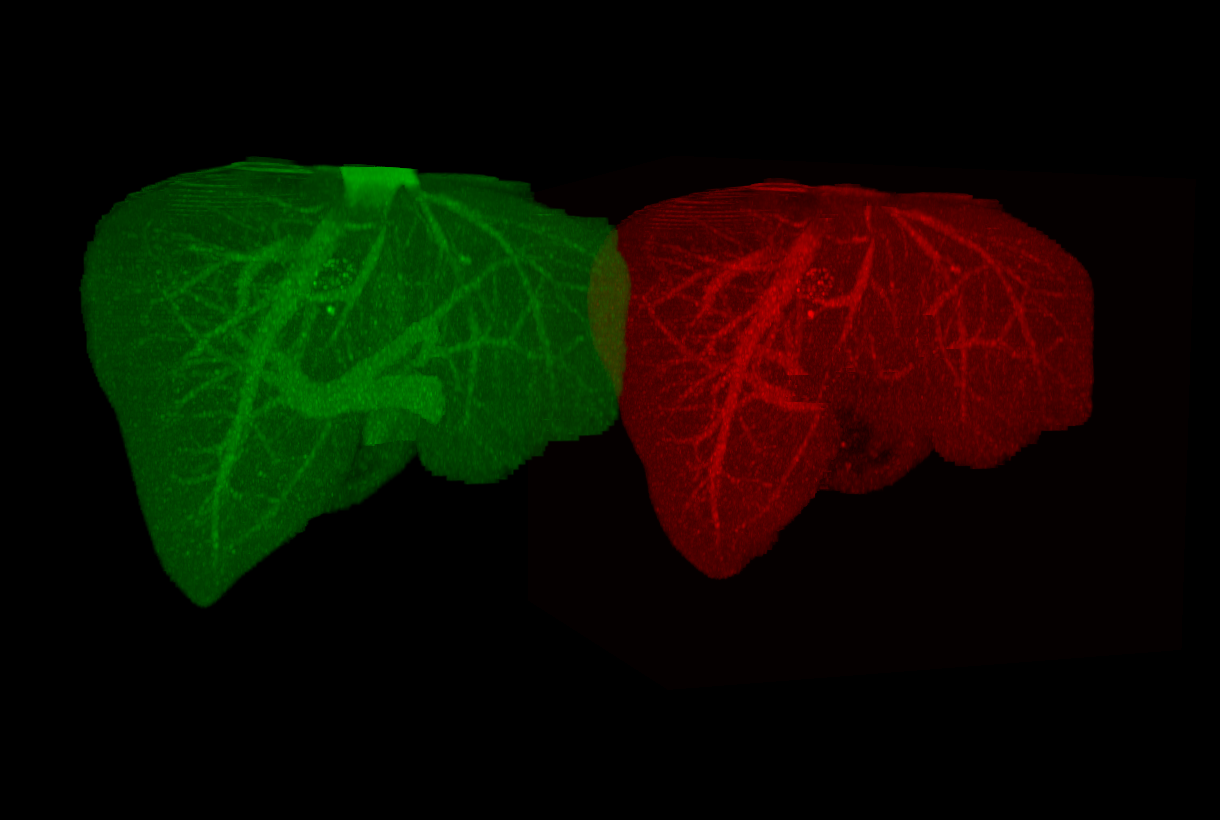
\includegraphics[height=5cm]{Images/ircad_corrected_gt.png}
  \caption{En rouge, masque du foie à la version 1. En vert, masque à la version 2 comprenant les veines portes et caves.}
  \label{fig:masques_globaux_ircad}
\end{figure}

\paragraph{VascuSynth}
Pour le jeu de données issu de VascuSynth, il n'y a pas d'organe réel. Le masque global est donc un masque recouvrant l'image entière. Nous aurions pu créer un masque artificiel et simuler des bordures d'organes. Cependant, cette problématique est déjà couverte par les deux autres bases de données. De plus, ceci nous permet d'évaluer la qualité du rehaussement sans la présence d'artefacts de bordure.

\paragraph{Bullitt}
Pour Bullitt, nous avons été confrontés à deux problèmes. Le premier est qu'il n'y avait pas de masques du cerveau pour cette base. Ces masques ont dû être créés manuellement pour les 33 volumes utilisés. Deuxièmement, nous avons dû faire face à un problème d'annotations. \newV{En effet, une partie des vaisseaux ne faisaient pas partie du périmètre d'étude de Sanchez et al. \cite{Sanchez2019_annotations_deep} (Fig. \ref{fig:masques_Bullitt}).} De larges veines dans la région périphérique intérieure du cerveau ne sont donc pas annotées. Celles-ci auraient été rehaussées lors de l'évaluation de nos filtres et auraient influencé négativement les résultats présentés dans le chapitre suivant. Nous avons donc choisi de réduire le masque du cerveau de manière à ignorer ces vaisseaux.

\begin{figure}[!ht]
  \centering
  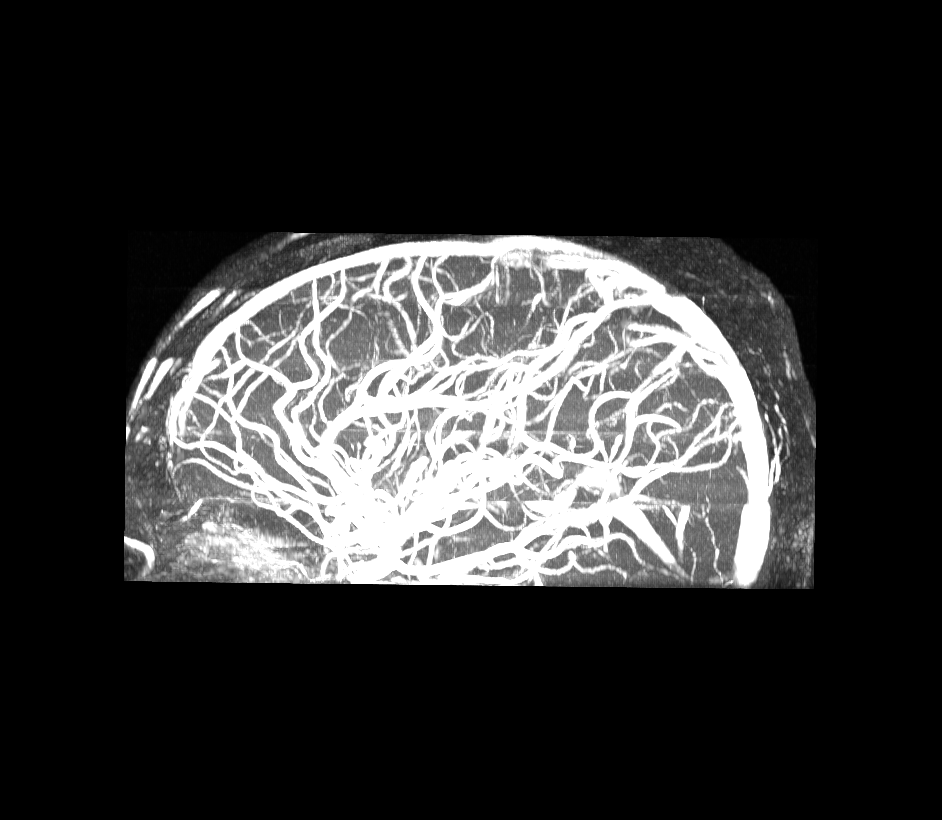
\includegraphics[height=4cm]{Images/bullitt_brain.png}
  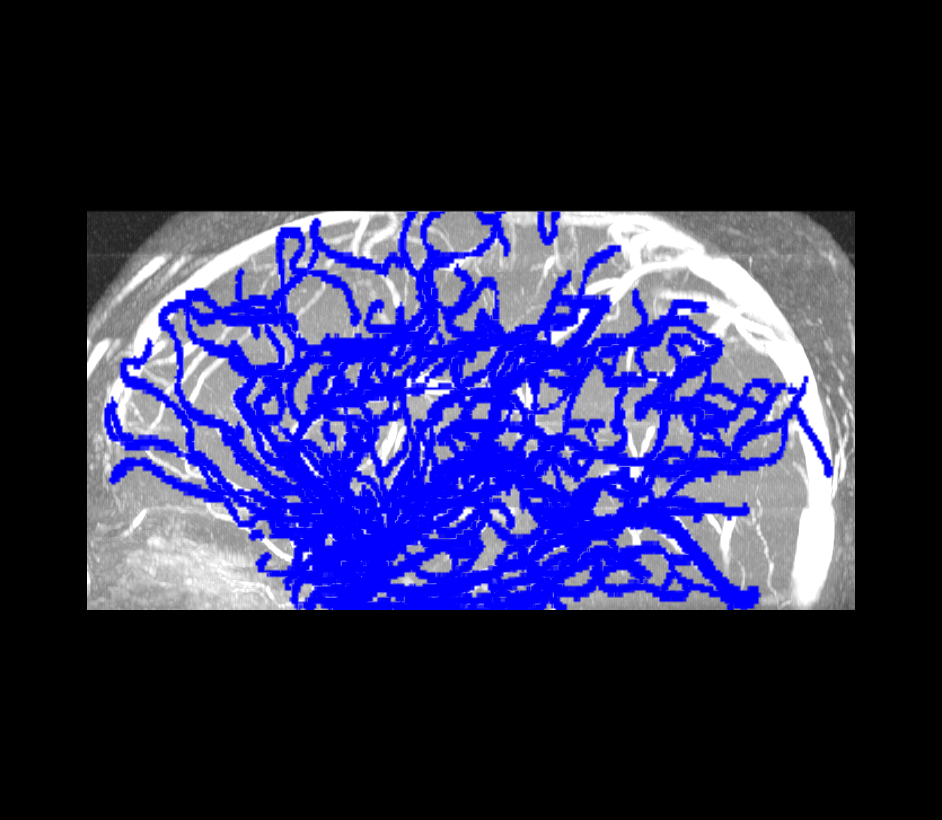
\includegraphics[height=4cm]{Images/bullitt_gt.png}
  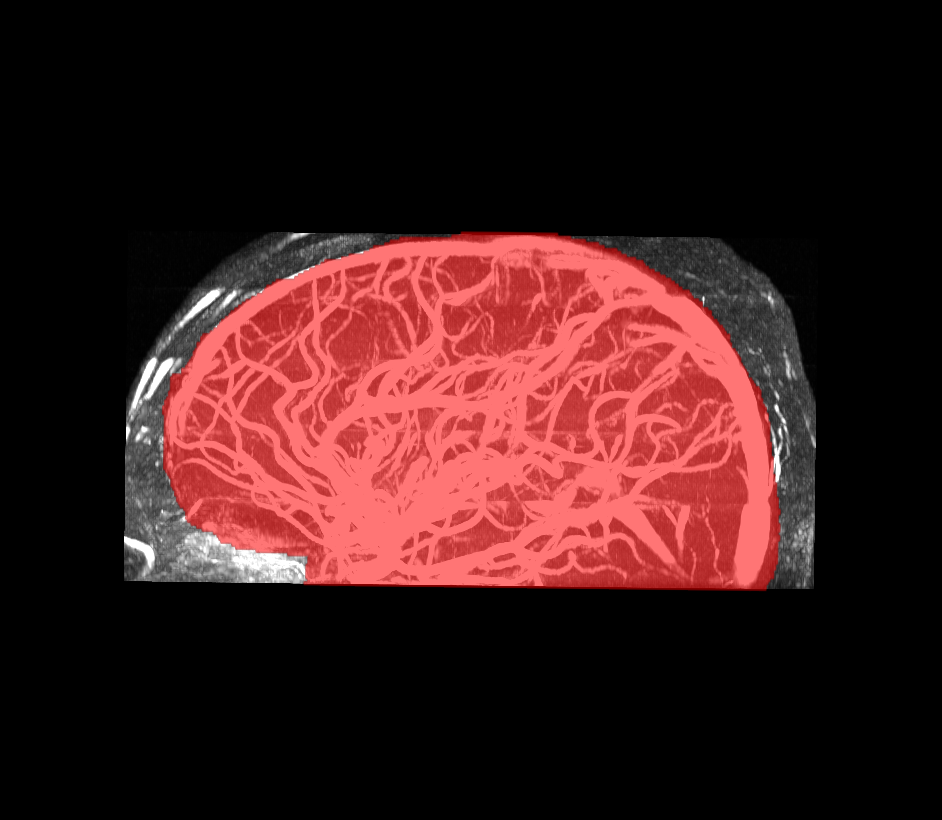
\includegraphics[height=4cm]{Images/bullitt_brainMask.png}
  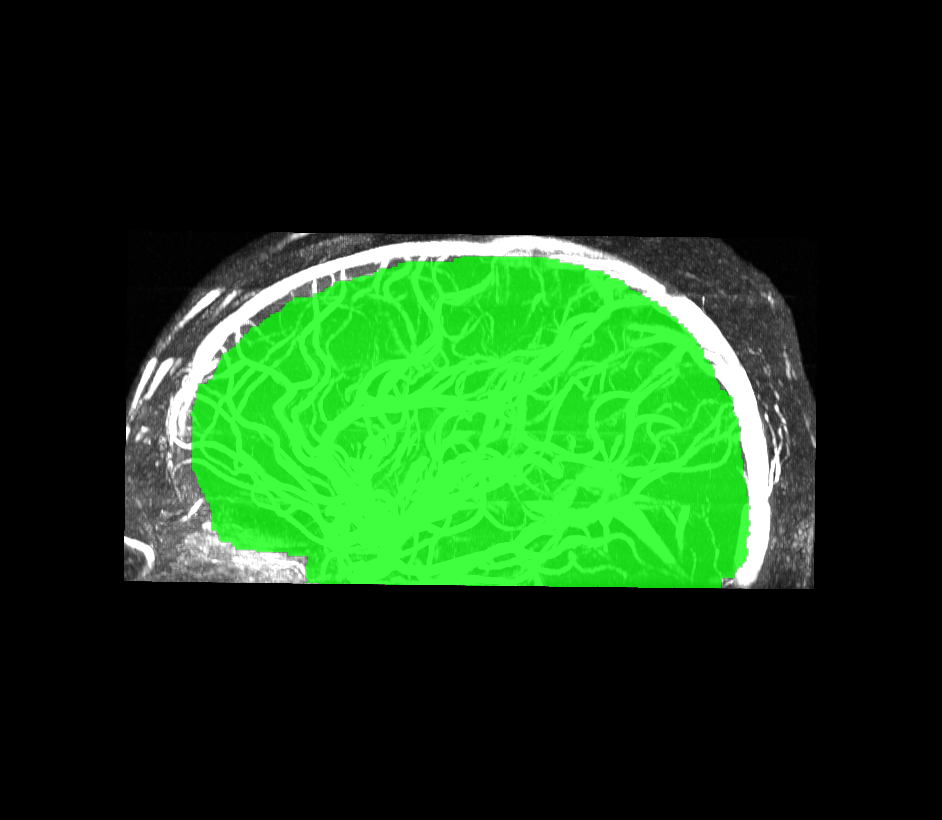
\includegraphics[height=4cm]{Images/bullitt_brainMask_ok.png}
  \caption{En blanc, MIP d'un cerveau. En bleu, vérité terrain des vaisseaux. En rouge, masque du cerveau et en vert, masque corrigé. Ce masque permet d'ignorer les vaisseaux non annotés tout en conservant le cercle de Willis situé à la base du cerveau.}
  \label{fig:masques_Bullitt}
\end{figure}

\newV{Nous avons redimensionné le masque du cerveau à $70$ \percent{} de sa taille initiale en conservant son centre à la même position. Ce premier masque recouvre une majorité du volume du cerveau en ignorant les veines non annotées. Néanmoins, il ne recouvre pas la zone fortement vascularisée, le cercle de Willis, au niveau de la bordure inférieure du masque. Pour conserver ces vaisseaux, nous avons redimensionné un second masque du cerveau à $40$ \percent{} de sa taille initiale. Nous avons ensuite utilisé l'intersection du premier masque et de la zone sous le second masque comme nouveau masque du cerveau (Fig. \ref{fig:masques_Bullitt_new}).}

\begin{figure}[!ht]
  \centering
  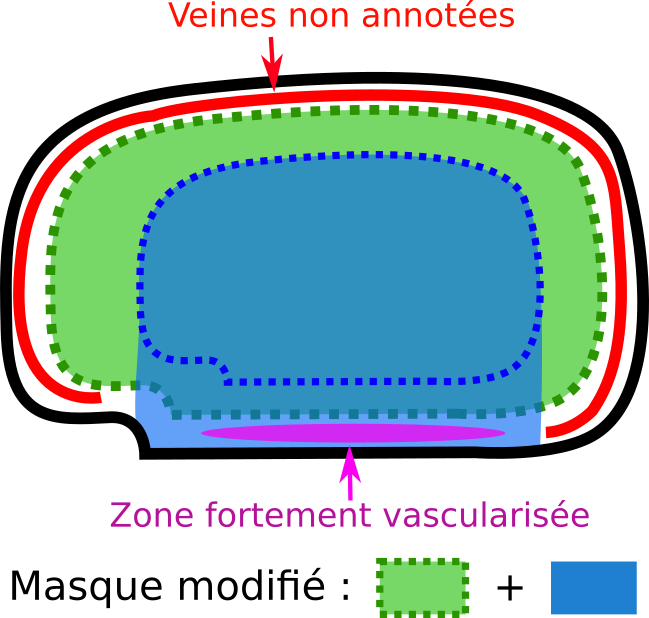
\includegraphics[height=6cm]{Images/bullitt_new_mask.png}
  \caption{Composition du nouveau masque du cerveau excluant les veines périphériques (rouge). Deux redimensions à $70$ \percent{} (vert) et $40$ \percent{} (bleu) de la taille initiale du masque du cerveau (noir) permettent de créer le masque final.}
  \label{fig:masques_Bullitt_new}
\end{figure}

\subsection{Masques des vaisseaux}
\subsubsection{Outils de simplification des vaisseaux}

\newV{La création des masques du voisinage des vaisseaux et du masque des bifurcations directement à partir de la vérité terrain voxélique des vaisseaux est complexe. Cette complexité est due au fait que plus la dimension d'un objet croit, plus il est difficile à décrire et à manipuler. Par exemple, une bifurcation est plus facile à définir sur une structure en quasi une dimension qu'une structure en 2D ou en 3D (Fig. \ref{fig:shape_abstraction}).}

\begin{figure}[!ht]
  \centering
  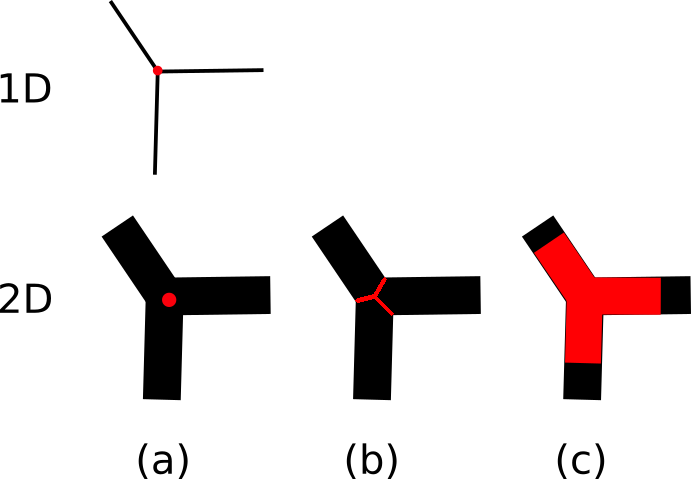
\includegraphics[height=6cm]{Images/shape_abstraction.png}
  \caption{Illustration de l'augmentation de la complexité de la description du concept de bifurcations avec l'augmentation de dimension. En 1D la bifurcation peut-être définie comme un point. En 2D, la position du point est plus incertaine et les manières de définir une bifurcation sont plus nombreuses.}
  \label{fig:shape_abstraction}
\end{figure}

\newV{Le squelette est le résultat d'un algorithme permettant d'affiner un objet binaire jusqu'à ce qu'il ne forme plus qu'une structure quasi 1D (Fig. \ref{fig:vascu_skeleton}). On peut visualiser le squelette comme étant le résultat d'une forme dont les bords ont été rongés au fur et à mesure et dont le processus s'arrête lorsque le fait d'enlever un voxel supplémentaire modifie la topologie de l'objet initial \cite{Lee1994_3D_skeleton}. Une autre manière de voir le squelette est de considérer la carte de distances internes à un objet où pour chaque voxel, on calcule la distance au bord le plus proche. Dans ce cas, l'ensemble des maxima locaux forme un ensemble d'arêtes connexes correspondant au squelette.}

\begin{figure}[!ht]
  \centering
  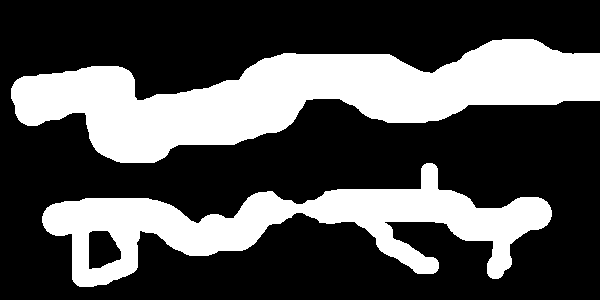
\includegraphics[height=4cm]{Images/skel_example.png}
  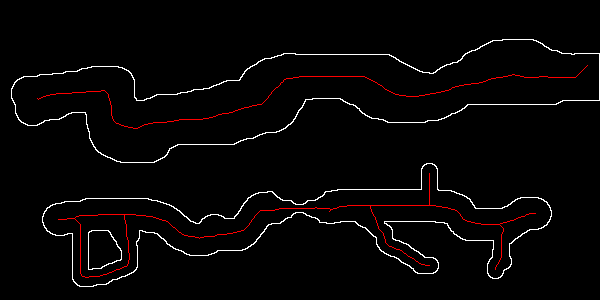
\includegraphics[height=4cm]{Images/skel.png}
  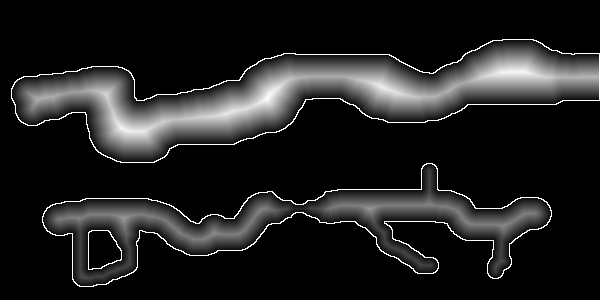
\includegraphics[height=4cm]{Images/skel_dt.png}
  \caption{De haut en bas : Image binaire, squelette de la structure et transformée en distance interne. Le squelette correspond aux crêtes formées par les maxima locaux.Le contour externe des structures est conservé pour plus de lisibilité.}
  \label{fig:vascu_skeleton}
\end{figure}

\newV{Les algorithmes de squelettisation dépendent de la connexité des voxels. En 2D on parle de 4-connexités lorsque l'on considère les pixels Nord, Sud, Est, Ouest et de 8-connexité en ajoutant les pixels situés sur les diagonales (Nord-Est, Nord-Ouest, Sud-Est, Sud-Ouest). L'équivalent 3D de la 4-connexité est la 6-connexité et l'équivalent 3D de la 8-connexité est la 26-connexité.}

\newV{L'algorithme proposé par ITK permet d'obtenir des squelettes 3D \cite{Homann2007_implementation_thinning} en 26-connexité afin d'obtenir des squelettes sans déconnexions.}

\newV{La squelettisation simplifie énormément l'identification des bifurcations ainsi que des différentes branches des vaisseaux comme nous allons le voir dans les sections qui suivent.}

\subsubsection{Masques des bifurcations}

Les bifurcations sont des zones décrites par la littérature comme particulièrement mal rehaussées par les filtres. Celles-ci sont toutefois étudiées de manière qualitative sur quelques exemples synthétiques. Cependant, très peu de travaux, aussi bien pour des données synthétiques que pour des données réelles, ont essayé de mesurer quantitativement le rehaussement sur les bifurcations des vaisseaux. Une des raisons plausibles est qu'il est difficile de définir une bifurcation de manière précise. Par exemple, si l'on considère la bifurcation comme un point, il est nécessaire d'estimer son positionnement. Si les vaisseaux ont la même taille, on peut prendre le croisement des lignes centrales. La question devient plus complexe sur des bifurcations avec des vaisseaux de taille différentes.

En observant des exemples qualitatifs de rehaussement des bifurcations dans des publications précédentes, on se rend compte que la perte de signal est graduelle. On obtient un signal relativement fort au niveau des vaisseaux qui diminue graduellement jusqu'au point de fusion des vaisseaux. C'est la mesure de cette perte graduelle qui nous intéresse. Notre masque de bifurcations doit donc non seulement couvrir le centre de celles-ci, mais aussi couvrir une partie des vaisseaux quittant la bifurcation (Fig. \ref{fig:shape_abstraction} (c)).

La localisation des bifurcations des vaisseaux est facilité par le squelette des vaisseaux. Une fois celui-ci obtenu, on peut caractériser chaque voxels par le nombre de voxels adjacents. Un seul voxel adjacent signifie la présence d'une extrémité, deux voxels adjacents indiquent que le voxel appartient à une branche. À partir de 3 voxels, le voxel appartient à une bifurcation.

On peut tout à fait automatiser cette tâche de comptage grâce à l'opérateur de convolution. Cela nécessite un squelette binaire avec un premier plan blanc (intensité de 1) sur fond noir (intensité 0) ainsi qu'un noyau de convolution rempli de 1. Il suffit alors de seuiller le résultat pour obtenir les bifurcations recherchées.

Une fois les bifurcations identifiées et localisées spatialement, on peut dilater ces voxels par un élément structurant afin d'obtenir une boule recouvrant les zones de bifurcations. On peut ensuite masquer cette boule par la segmentation originale pour obtenir une segmentation des bifurcations en forme de fourche (Fig. \ref{fig:bifurcations_masks}).

\begin{figure}[!ht]
  \centering
  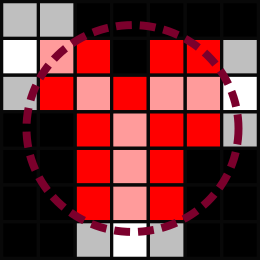
\includegraphics[height=4cm]{Images/bifurcation_creation.png}
  \caption{Création du masque des bifurcations. Les vaisseaux apparaissent en gris et leur squelette en blanc. La zone d'intérêt de la bifurcation (rouge) est composée par l'intersection entre une boule et la vérité terrain des vaisseaux. Le diamètre de la boule est défini en fonction de la taille des bifurcations.}
  \label{fig:barbelures}
\end{figure}

\begin{figure}[!ht]
  \captionsetup[subfigure]{justification=centering}
  \begin{subfigure}{0.45\textwidth}
    \centering
    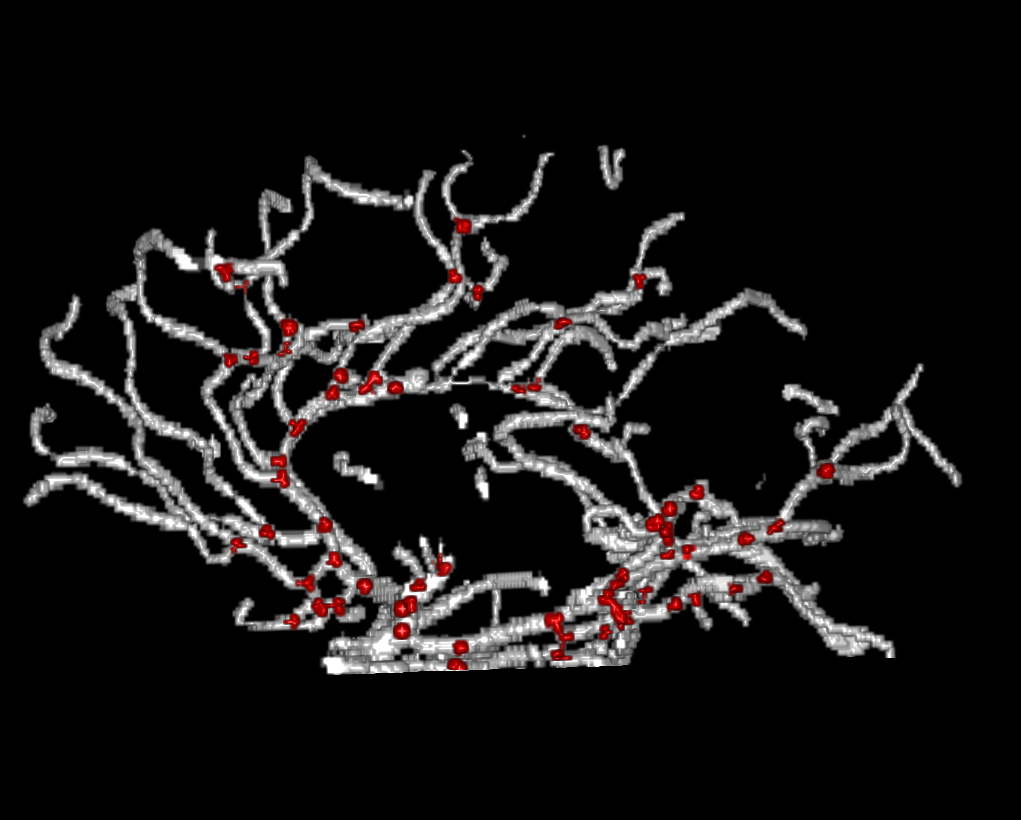
\includegraphics[height=5cm]{Images/bifurcations_bullitt.png}
    \caption{Bullitt}
  \end{subfigure}
  \begin{subfigure}{0.45\textwidth}
    \centering
    \adjincludegraphics[height=5cm,trim={{0.25\width} {0.25\height} {0.2\width} {0.05\height}},clip]{Images/bifurcations_vascu.png}
    \caption{VascuSynth}
  \end{subfigure}
  \\
  \centering
  \begin{subfigure}{0.45\textwidth}
    \centering
    \adjincludegraphics[width=\textwidth,trim={{0.1\width} {0.15\height} {0.1\width} {0.1\height}},clip]{Images/bifurcations_ircad.png}
    \caption{Ircad}
  \end{subfigure}
  \caption{Masque des bifurcations (rouge) pour les trois jeux de données}
  \label{fig:bifurcations_masks}
\end{figure}

Cette méthode, censée fonctionner en théorie produit de mauvais résultats avec l'algorithme de squelettisation d'ITK. En 26-connexité, Une bifurcation peut-être définie comme 3 voxels au lieu d'un seul, par effet miroir de notre définition d'une bifurcation (Fig. \ref{fig:skel_illustration} (b) ). Cette observation n'est pas problématique au niveau de la géométrie des vérités terrains finales, mais triple le temps de traitement pour ces bifurcations.

Plus problématique, la nature du squelette d'ITK peut-être localement en 4-connexité. Nous détectons donc des bifurcations à des endroits où il n'en existe pas (Fig. \ref{fig:skel_illustration} (c) ). 

\begin{figure}[!ht]
  \captionsetup[subfigure]{justification=centering}
  \centering
  \begin{subfigure}{0.32\textwidth}
    \centering
    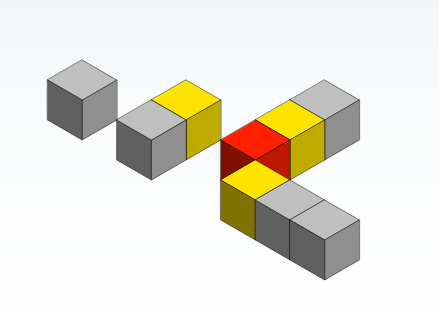
\includegraphics[width=\textwidth]{Images/problem_skel0.png}
    \caption{}
  \end{subfigure}
  \begin{subfigure}{0.32\textwidth}
    \centering
    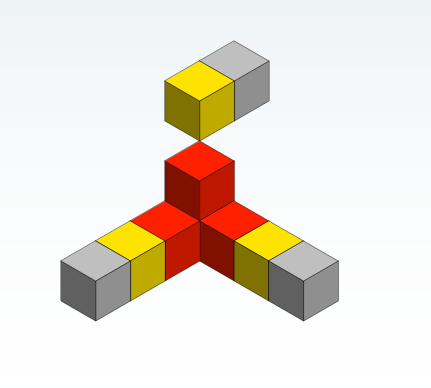
\includegraphics[width=\textwidth]{Images/problem_skel3.png}
    \caption{}
  \end{subfigure}
  \begin{subfigure}{0.32\textwidth}
    \centering
    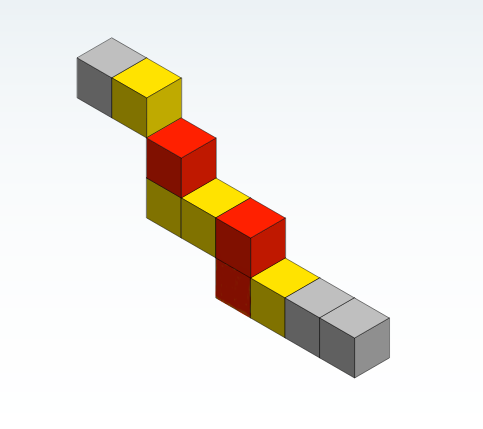
\includegraphics[width=\textwidth]{Images/problem_skel2.png}
    \caption{}
  \end{subfigure}

  \caption{Exemples de squelettes rencontrés avec l'algorithme de squelettisation 3D d'ITK en 26 connexités. En rouge voxels ayant exactement 3 voisins (jaune). Lorsque les courbures du squelette s'effectuent en 4-connexité, des voxels peuvent être identifiés comme des bifurcations (b) et (c).}
  \label{fig:skel_illustration}
\end{figure}

On peut aussi observer que les irrégularités sur la surface des vaisseaux produisent des branches parasites du squelette et donc créé des bifurcations sur le squelette, mais inexistantes au niveau des vaisseaux (Fig. \ref{fig:barbelures}). Ces branches supplémentaires sont difficiles à identifier par rapport au squelette légitime. Ce problème n'est cependant significatif que pour les gros vaisseaux de la base de l'Ircad et nous l'atténuons en conservant les bifurcations seulement à l'intérieur du masque original du foie (sans les troncs manuellement ajoutés).

\begin{figure}[!ht]
  \centering
  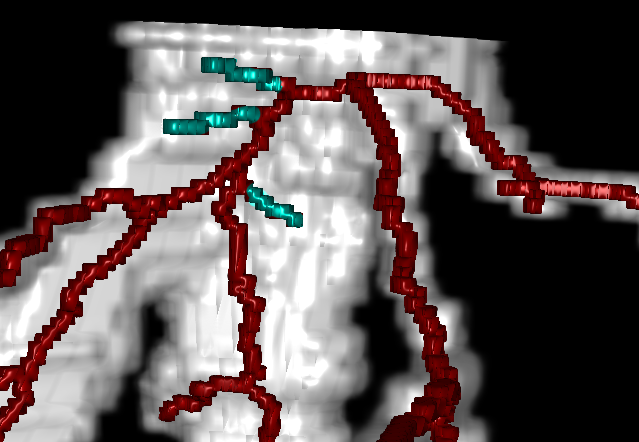
\includegraphics[height=4cm]{Images/barbelures.png}
  \caption{Partie supérieure de la veine hépatique à l'entrée d'un foie de l'Ircad. Les irrégularités sur la surface des vaisseaux provoquent des branches parasites pour la détection des bifurcations des vaisseaux (bleu).}
  \label{fig:barbelures}
\end{figure}


Les problèmes précédents ont ensuite été réglés en partie dans une seconde itération. Nous avons pu produire des squelettes plus propres à partir d'un algorithme de squelettisation par noyau critique \cite{Bertrand2006_critical_kernel} et ainsi éliminer une grande partie des bifurcations erronées (Fig. \ref{fig:skel_illustration} (c) ).

\newV{Dans cette seconde itération avec un squelette de meilleure qualité, nous avons aussi abandonné l'identification des bifurcations par convolution pour utiliser une méthode à base de parcours de graphe. Le parcours de graphe permet à la fois de détecter les bifurcations, de nettoyer les cas miroirs et de labelliser chaque branche du réseau vasculaire en fonction de sa taille. Le fonctionnement du parcours de graphe est expliqué dans la section suivante dans laquelle nous décrivons la construction des parcours par taille.}

\subsection{Masques par taille}

\newV{Dans un réseau vasculaire, chaque branche n'est pas constituée du même nombre de voxels. L'ordre de grandeur pour les gros vaisseaux est d'une dizaine de voxels de diamètres pour une centaine de long. L'ordre de grandeur pour les petits vaisseaux est de quelques voxels de diamètre pour une dizaine de voxels de long. Chaque image présente une répartition différente entre gros et petits vaisseaux. Si l'on calcule des métriques quantitatives sur la zone d'intérêt du voisinage du réseau vasculaire total, il est impossible de connaître le poids d'un des trois types de vaisseaux dans le calcul de la métrique d'évaluation. Il est toutefois possible qu'un filtre produise un rehaussement différent selon la taille des vaisseaux. C'est pourquoi nous avons décidé de créer une partition de ce masque de voisinage global en classes dépendant de la taille des vaisseaux.}

Créer une partition des vaisseaux par taille revient à labelliser chaque branche en fonction de son diamètre puis à classifier les branches par taille. Comme pour les bifurcations, nous sommes partis du squelette de la vérité terrain des vaisseaux.

\newV{Le parcours du squelette de proche en proche nous permet de déterminer la hiérarchie des branches. Pour cela, on définit les voxels du squelette comme un graphe dans lequel les voxels sont les nœuds et les arrêtes sont définies par adjacence des voxels en 26-connexité (Fig. \ref{fig:adjacence}).}

\begin{figure}[!ht]
  \centering
  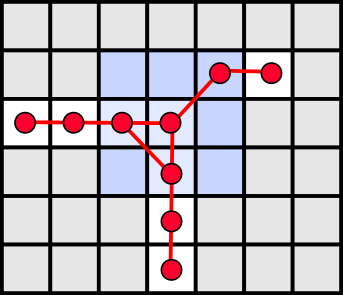
\includegraphics[height=4cm]{Images/graph_construct.png}
  \caption{Représentation 2D du graphe (rouge) construit à partir du squelette (blanc). Les voxels forment les nœuds du graphe et les arêtes sont définies par l'adjacence en 26-connexité des voxels (bleu).}
  \label{fig:adjacence}
\end{figure}

\newV{Il est tout à fait possible que des déconnexions entre les vaisseaux existent dans les vérités terrains. Les traitements de parcours de graphe que nous décrivons sont donc réalisé pour chaque composante connexe.}

\newV{Une première étape consiste à identifier un point de départ sur une composante connexe. Nous avons choisi comme point de départ le point sur le squelette où le diamètre des vaisseaux est le plus élevé. Il correspond à un point habituellement au centre du vaisseau racine pour les réseaux vasculaires en forme d'arbres (Ircad et VascuSynth). Pour identifier la position du nœud de départ, nous utilisons la transformée en distance interne à la vérité terrain des vaisseaux. }

\newV{Celle-ci nous permet d'obtenir la distance aux bords de tous les pixels de la segmentation. À branches parasites près, le squelette correspond à la ligne centrale des vaisseaux ; la valeur de la carte de distance pour les points du squelette correspond alors au rayon des vaisseaux. Nous choisissons donc comme point de départ le voxel du squelette avec le rayon le plus large (Fig. \ref{fig:graph_traversal_starter}).}

\begin{figure}[!ht]
  \centering
  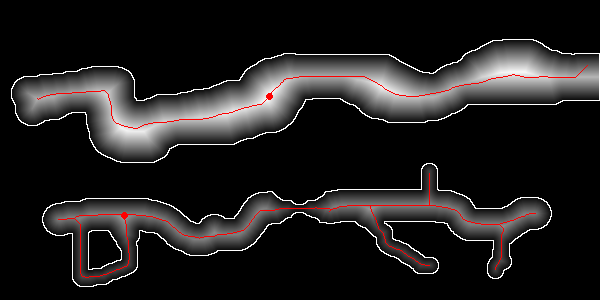
\includegraphics[height=4cm]{Images/skel_seed.png}
  \caption{Le départ du parcours de graphe est le point sur le squelette (rouge) où la valeur de la carte de distance est la plus élevée. Les valeurs de la carte de distance sur le squelette correspondent au diamètre des vaisseaux.}
  \label{fig:graph_traversal_starter}
\end{figure}

\newV{Un label est ensuite propagé le long du squelette jusqu'à la rencontre de la prochaine bifurcation, c'est-à-dire un voxel avec plus de deux voisins, ou d'une extrémité. Le voxel d'initialisation est un cas particulier puisqu'il est souvent détecté au centre d'une branche. La branche racine du squelette est donc visitée par deux fronts de propagation portant le même label contrairement aux autres branches qui ne sont visitées que par un seul front. À chaque rencontre d'une bifurcation, un nouveau label unique est associé à une nouvelle branche (Fig. \ref{fig:graph_traversal} (a)).}

\begin{figure}[!ht]
  \centering
  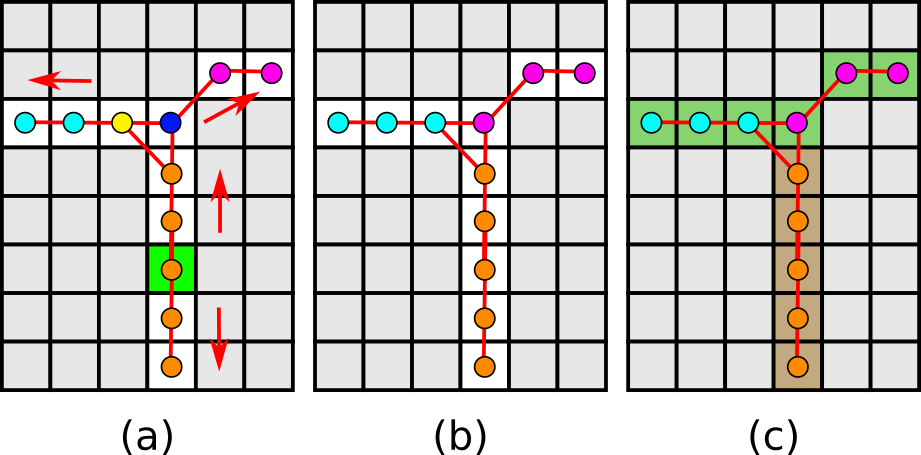
\includegraphics[width=\textwidth]{Images/vessels_size_creation.png}
  \caption{ (a) Le parcours de graphe pour la labellisation des vaisseaux commence à la racine (vert). La labellisation est ensuite propagée de proche en proche. Le label change lorsqu'une bifurcation (un nœud avec plus de deux voisins) est découverte. (b) Les labels isolés sont fusionnés avec le label d'une des branches adjacente. (c) On associe ensuite au squelette de chaque branche une classe qui est propagée sur les voxels de la vérité terrain.}
  \label{fig:graph_traversal}
\end{figure}


Cette méthode souffre du même défaut que pour la création des masques de bifurcations à cause de la symétrie de configuration rencontrée sur les bifurcations (cycle du graphe Fig. \ref{fig:adjacence}). Cette symétrie provoque l'apparition de labels pour lesquels seulement 1 voxel leur est attribué (Fig. \ref{fig:graph_traversal} (a)). Une solution est donc de relabelliser ces voxels avec le label d'une branche adjacente. Cela n'impacte pas le résultat final. Cette méthode de relabellisation de branches de petites tailles (moins de 4-5 voxels) peut aussi être utilisée si un algorithme de squelettisation moins performant est utilisé.

\begin{figure}[!ht]
  \centering
  \adjincludegraphics[width=0.60\textwidth,trim={{0\width} {0.2\height} {0\width} {0\height}},clip]{Images/vs_labels.png}
  \\
  \adjincludegraphics[width=0.60\textwidth,trim={{0\width} {0.2\height} {0\width} {0\height}},clip]{Images/vs_labelMask.png}
  \caption{En haut, taille des vaisseaux par branche : Une branche est caractérisée par son rayon maximal. Les vaisseaux de faible diamètre sont représenté en bleu et les vaisseaux de gros diamètres en rouge. En bas, partition en trois classes des vaisseaux : gros vaisseaux en marron, vaisseaux moyens en jaune et petits vaisseaux en vert.}
  \label{fig:vessels_partition}
\end{figure}

Une fois les branches du squelette labellisées, celles-ci doivent être relabellisées par la taille des branches des vaisseaux (Fig. \ref{fig:vessels_partition}). Pour cela nous définissons leur taille comme étant le rayon maximum de la branche obtenue grâce à la carte de distance précédemment calculée. Enfin, il est possible de propager les labels générés sur le squelette à l'ensemble des voxels en utilisant un algorithme de \textit{fast marching} ou des cellules de Voronoï avec les labels pour graines (Fig. \ref{fig:voronoi}). Le choix du rayon maximum plutôt que le rayon moyen des branches assure que la limite des partitions des masques par taille soit bien définie.

\begin{figure}[!ht]
  \centering
  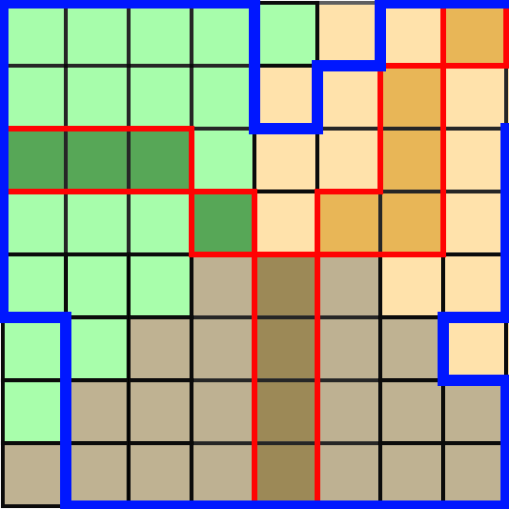
\includegraphics[height=4cm]{Images/voronoi.png}
  \caption{Propagation des labels du squelette (zone rouge) sur les vaisseaux (zone bleu) par calcul de leur zone d'influence grâce à l'algorithme des cellules de Voronoï. Chaque voxel est labellisé par le label du squelette le plus proche. Lorsque un voxel est à équidistance d'un label, une décision arbitraire est prise.}
  \label{fig:voronoi}
\end{figure}

Le masque du voisinage des vaisseaux est construit en fonction du diamètre des vaisseaux minimal, moyen et maximal de chaque jeu de données : $[0,3]$, $]3,6[$ et $]6,\inf[$ mm pour l'Ircad et $[0,1]$, $]1,2[$ et $]2,\inf[$ mm pour VascuSynth. Le diamètre des vaisseaux dans le jeu de données Bullitt varie peu ; nous avons donc utilisé deux masques seulement : $[0,0.513]$ mm (\maskvesselSmall) et $]0.513,\inf[$ mm (\maskvesselMedium). Le masque du voisinage des vaisseaux (\maskvessel) et ses partitions (\maskvesselLarge,\maskvesselMedium,\maskvesselSmall) sont obtenus par dilatation de la vérité terrain des vaisseaux en fonction de leur diamètre. Ces valeurs ont été déterminées empiriquement, 9, 7, 5 voxels pour le jeu de l'Ircad, 5, 3 pour le jeu Bullitt et 7, 5, 3 pour VascuSynth. Lorsque deux masques de voisinages se chevauchent, la région conflictuelle est attribuée au masque des vaisseaux les plus larges. On garantit ainsi que les trois masques constituent bien une partition de $\maskvascular$ tout en préservant la cohérence des subdivisions créées (Fig. \ref{fig:vs_masks} et \ref{fig:numibranch}).

\begin{figure}[!ht]
  \centering
  \includegraphics[height=3cm]{Images/numibranch.png}
  \caption{Illustration de la hiérarchie de la partition des zones d'intérêts par tailles. Les zones d'intérêts les plus grandes ont précédence sur les zones les plus petites. Les zones d'intersections sont donc attribuées à la zone la plus grande, on évite ainsi que des voxels participent à plusieurs zones d'intérêts.}
  \label{fig:numibranch}
\end{figure}


En particulier, nous avons $\maskbif \subseteq \maskvascular \subseteq \maskglobal$ et $\maskvascular = \maskvesselLarge \cup \maskvesselMedium \cup \maskvesselSmall$.

\begin{figure}[!ht]
  \centering
  \adjincludegraphics[width=0.45\textwidth,trim={{0\width} {0.2\height} {0\width} {0\height}},clip]{Images/vs_gt.png}
  \adjincludegraphics[width=0.45\textwidth,trim={{0\width} {0.2\height} {0\width} {0\height}},clip]{Images/vs_gt_liver.png}
  \adjincludegraphics[width=0.45\textwidth,trim={{0\width} {0.2\height} {0\width} {0\height}},clip]{Images/vs_VN.png}
  \adjincludegraphics[width=0.45\textwidth,trim={{0\width} {0.2\height} {0\width} {0\height}},clip]{Images/vs_large.png}
  \adjincludegraphics[width=0.45\textwidth,trim={{0\width} {0.2\height} {0\width} {0\height}},clip]{Images/vs_medium.png}
  \adjincludegraphics[width=0.45\textwidth,trim={{0\width} {0.2\height} {0\width} {0\height}},clip]{Images/vs_small.png}
  \caption{Zones d'intérêts (ZI) utilisés dans notre banc de test. Vérité terrain (blanc), ZI de l'organe (vert), ZI du voisinage des vaisseaux global (magenta), ZI du voisinage local des vaisseaux : large (rouge), moyen (cyan), petits (jaune)}
  \label{fig:vs_masks}
\end{figure}

Le masque \maskbif est construit à partir des positions des bifurcations extraites du squelette. Ces points sont ensuite dilatés par un facteur $kp$ où $p$ est le rayon des vaisseaux et $k=3$ si $p\leq 1$ voxel et 2 sinon. L'intersection avec la vérité terrain est ensuite réalisée de manière à assurer que \maskbif est inclus dans les vaisseaux.
% Finir sur la gestion et la taille des voisinages


\begin{table}
  \begin{center}
    \resizebox{\textwidth}{!}{
      \begin{tabular}{l|l|l|l}
          \hline
          Propriétés                      &  Version 1 (ICPR)       & Version 2 (TMI) \\ \hline  \hline 
          Bases de données                & Ircad, VascuSynth       & Ircad, VascuSynth, Bullitt \\ \hline
          Isotropie des données réelles   & [1mm,1mm,1mm]           & [maxRes,maxRes,maxRes] \\ \hline
          Dynamique d'intensité des images synthétiques  & Manuelle & Mesures sur images réelles \\ \hline
          Artefacts d'images synthétiques & Bruit, inhomogénéité    & Bruit, inhomogénéité, artefacts gaussiens   \\ \hline
          Bruit ricien pour images synthétiques  & 5,10,20          & 2,4,6 \\ \hline
          Masques & Organe, voisinage global, bifurcations & Organe, voisinage par taille, bifurcations \\
          Nombre de seuils & 100 & 200 \\ \hline  
      \end{tabular}
    }
  \end{center}
  \caption{Récapitulatif des paramètres des bases de données utilisés pour chaque version de nos expériences. Chaque version a donné lieu à une publication dont le contexte est fourni dans le chapitre \chapReproN{}.}
  \label{Tab:recap_versions}
\end{table}

\section{Description du banc de test}
\subsection{Fonctionnement global}
Notre banc de test est implémenté en deux blocs. Il est composé d'un premier bloc de calcul des métriques et d'un second bloc d'analyse des métriques récoltées.

Le premier bloc nécessite une base de données d'images et de leur vérité terrain, une liste de filtres, une liste de jeux de paramètres par filtres, un ensemble de zones d'intérêts et d'une série de métriques. L'algorithme est détaillé en algorithme \ref{alg:BenchmarkStep}.

\begin{algorithm}[!ht]
  \caption{Algorithme du banc de test}\label{alg:BenchmarkStep}
      \textbf{Entrée :}
      Ensemble des images $I=\{I_1,\ldots,I_N\}$ \\
      Ensemble des vérités terrains $GT=\{GT_1,\ldots,GT_N\}$\\
      Filtre $F$\\
      Régions d'intérêt $ROI$\\
      Jeu de paramètres  $P=\{ P_{scale},P_{intr} \} $ du filtre F\\ 
      Métriques $M$\\
      Nombre de seuils $S$ \\
      \textbf{Algorithme :}
      \begin{algorithmic}
          \For{$i$ in $[1,N]$}
              \State $R_{i} \gets AppliquerFiltre(F,I_i,P)$
              \For{$s$ in $[1,S]$}
                \State $RS_{i} \gets Seuiller(R_{i},s)$
                \State $RS_{i}^{masked},GT_{i}^{masked} \gets AppliquerROI( RS_{i},GT_{i}, ROI ) $
                \State $m_{i} \gets CalculerMétriques(RS_{i}^{masked}, GT_{i}^{masked}, M)$
                \State $SauvegarderMétriques(F,P,I_i,ROI)$
              \EndFor
          \EndFor
      \end{algorithmic}
      %\textbf{Sortie:}\\ Mean metric value  $\frac{1}{N}\sum_i{m_i}$
  \end{algorithm}

Pour chaque volume de la base, chaque filtre et chaque paramètre, un filtrage est réalisé. Ce filtrage est ensuite seuillé afin de le comparer à la vérité terrain du volume. Afin de ne pas choisir arbitrairement un seuil, nous effectuons un ensemble de seuils successifs répartis linéairement dans $[0,1]$ et dont le nombre est choisi par l'utilisateur. Ensuite, pour chaque zone d'intérêt, une série de métriques toutes basées sur le calcul de la matrice de confusion entre chaque paire $\{volume Binaire, vérité Terrain\}$ sont calculées. Les résultats sont ensuite stockés dans un fichier par zone d'intérêt.

Les nombres de seuils et les métriques utilisées sont définies dans le chapitre suivant qui détaille nos expériences. 

Le second bloc est un bloc d'analyse des métriques. Il prend en entrée les fichiers de zones d'intérêt, sous forme de fichier csv, et permet d'exprimer les métriques en termes de moyennes par volumes et par zones d'intérêt et de construire des rapports sous forme de tableaux et de graphes de résultats (Fig. \ref{fig:bench_module2}). Le fonctionnement de ce second bloc est détaillé dans le chapitre suivant dans la partie détaillant l'optimisation des paramètres. 

\begin{figure}[!ht]
  \centering
  \includegraphics[height=6cm]{Images/bench_Ircad_PS_MCC.pdf}
  \includegraphics[height=6cm]{Images/bench_Ircad_ROC.pdf}
  \includegraphics[width=\textwidth]{Images/bench_type_of_results.png}
  \caption{Sortie type du second module. Les résultats numériques sous forme de tableaux sont aussi compilés sous forme de graphiques.}
  \label{fig:bench_module2}
\end{figure}

\subsection{Considérations sur les performances}

Le découplage en deux blocs pour rendre indépendant la collecte des métriques et l'analyse de celles-ci permet un travail hors ligne et offre plus de modularité, puisque le module d'analyse peut-être interchangé selon les besoins de l'utilisateur. 

Une expérience peut très vite consommer des ressources importantes. À l'exécution, le bloc de calcul des métriques est en lui-même peu gourmand en ressources, il contient la vérité terrain du volume en cours, le résultat des filtrages, la zone d'intérêt courante et les pointeurs sur les fichiers de métriques (1 par zone d'intérêt). Le lancement des filtres peut être coûteux, car les mécanismes multi-échelles multiplient les volumes gardés en mémoire. Par exemple, pour les filtres à base de hessienne, il y a au minimum le volume d'entrée, les volumes représentant la matrice hessienne et le volume résultat du rehaussement. Si les images d'entrées sont larges, la demande en RAM peut rapidement dépasser plus de 10 Go en explorant 3 à 4 échelles de vaisseaux. 

En termes de stockage des résultats, le banc de test peut produire des volumes de données importants. Par exemple, tester une quarantaine de jeux de paramètres pour les 7 filtres et garder les volumes de résultats revient à multiplier le nombre de volumes sur disque par 280. 

Nous avons donc implémenté une option permettant de supprimer un volume de filtrage après que toutes les métriques ont été calculées. Le résultat d'une session de collecte des métriques n'est alors composé que de fichiers CSV en quelques mégabits et quelques dizaines de mégabits pour les plus gros. Nous avons aussi implémenté une option permettant de calculer des métriques à partir d'une base existante de filtrages. Lorsque l'espace disque est disponible, cela permet un gain de temps considérable puisque les filtrages n'ont pas besoin d'être recalculés afin d'évaluer de nouvelles métriques ou de nouvelles zones d'intérêt.

\newV{En termes de temps d'exécution, il était indispensable que le calcul des filtres soient l'unique goulot d'étranglement du premier bloc de l'application}. Nous avons donc été attentif à ce qu'aucune autre étape ne ralentisse inutilement le banc de test. Dans ce bloc, l'opération la plus coûteuse est le calcul du seuillage.

Dans une première version, nous avons utilisé un seuillage classique disponible dans ITK. Cependant, l'utilisation de ce filtre s'est avéré très coûteux en temps d'exécution dans le cadre de seuillages multiples. En effet, pour $N$ seuillages successifs de 1 à 0, un voxel seuillé à une valeur haute (par exemple 0.9) fera nécessairement partie de la segmentation pour tous les seuils inférieurs, il n'est donc pas nécessaire de les parcourir plusieurs fois. Dans le cas naïf, tous les pixels sont visités $N$ fois.

Dans une seconde version, nous proposons de réduire le nombre de visites d'un voxel de l'image pour calculer les 4 valeurs de la matrice de confusion pour chaque seuil : vrais positifs (VP), vrais négatifs (VN), faux positifs (FP) et faux négatifs (FN)~(Alg. (\ref{alg:BenchmarkThreshold})).

\clearpage

\scalebox{0.75}{
\begin{minipage}{0.75\linewidth}

\begin{algorithm}[H]
  \caption{
  Algorithme du seuillage}\label{alg:BenchmarkThreshold}
    \textbf{Entrée:}\\
      Image résultat d'un filtre $I$ \newV{d'indice $N$}\\
      Vérité terrain $VT$\\
      Valeurs de matrice de confusion initiales $VN_{init},VP_{init},FN_{init},FP_{init}$\\
      Valeurs de matrice de confusion par seuil $VN_{s},VP_{s},FN_{s},FP_{s}$\\
      Pas $p$ \\
      Liste d'indices des voxels $L^{ind}$ \\
      Liste d'intensités des voxels $L^{vi}$ \\
      \textbf{Algorithme:}
      %\resizebox{!}{\textheight}{
      \begin{algorithmic}
          \State $VN_{init},VP_{init},FN_{init},FP_{init} \gets 0 $
          \State $VN_{s},VP_{s},FN_{s},FP_{s} \gets 0$

          \For {$i \in 1...N$}
              \If {$ I(i) = 0 $}
                \If {$ GT(i) = 0 $}
                  \State $FN_{init} \gets FN_{init} + 1$
                \Else
                  \State $TN_{init} \gets TN_{init} + 1$
                \EndIf
              \Else
                \State $ AjouterIndexe(I_{i},L^{ind})  $
                \State $ AjouterIntensite(I_{i},L^{vi})$
              \EndIf
          \EndFor
          \State $t \gets 1$

          \While {$t \geq 0$}
            \While {$L^{ind} \neq \emptyset$}
              % We only have positives voxels
              \If {$ I(i) \geq t $}
                \If {$ GT(i) \geq 0 $}
                  \State $TP_{s} \gets TP_{s} + 1$
                  \Else
                  \State $FP_{s} \gets FP_{init} + 1$
                \EndIf
                
                \State $RetirerIndexe(I_{i},L^{ind})$
                \State $RetirerIntensite(I_{i},L^{vi})$
              \Else
                \If {$ GT(i) \geq 0 $}
                  \State $FN_{s} \gets FN_{s} + 1$
                \Else
                  \State $TN_{s} \gets TN_{init} + 1$
                \EndIf
              \EndIf
            \EndWhile

            \State  $ m \gets CalculerMetriques(TP_{init}+TP{s},TN_{init}+TN{s},FP_{init}+FP{s},FP_{init}+FP{s})$
            \State  $ SauvegarderMetriques(I,t,m)$
            \State $ t \gets t - p$ 
               
          \EndWhile
      \end{algorithmic}
  %}

      %\textbf{Output:}\\ Moyenne des métriques $\frac{1}{N}\sum_i{m_i}$
  \end{algorithm}
\end{minipage}
}

% Adaption aux besoins en mémoire de la machine
% Economie en calculs 

%\section{Expériences}
%\label{sec:Benchmark:experiences}

%\subsection{Stratégie d'optimisation}
%\label{sec:Benchmark:optimisation}

%\subsubsection{Optimisation globale}
%\label{sec:Benchmark:optimisation_globale}

%\subsubsection{Optimisation globale améliorée}
%\label{sec:Benchmark:optimisation_globale_ameliorée}

%\subsection{Résultats}
%\label{sec:Benchmark:résultats}

%\subsection{Reproductibilité}
%\label{sec:Benchmark:reproductibilité}

